\documentclass[12pt, letterpaper]{article}

\usepackage[utf8]{inputenc}
\usepackage[framemethod=TikZ]{mdframed}
\usepackage[hidelinks]{hyperref}
\usepackage{mathtools, amssymb, amsmath, cleveref, fancyhdr, geometry, tcolorbox, graphicx, float, subfigure, arydshln, url, setspace, framed, pifont, physics, ntheorem, cancel, mathrsfs}


%%% for coding %%%
\usepackage{listings}
\usepackage[ruled, vlined, linesnumbered]{algorithm2e}
\SetKwComment{Comment}{/* }{ */}
\newcommand\mycommfont[1]{\small\ttfamily\textcolor{mygreen}{#1}}
\SetCommentSty{mycommfont}

\geometry{letterpaper, left=2cm, right=2cm, bottom=2cm, top=2cm}

\pagestyle{fancy}
\fancyhead{}
\fancyhead[L]{\leftmark}
\fancyhead[R]{\rightmark}
\fancyfoot{}
\fancyfoot[C]{\thepage}
%\rfoot{\footnotesize  Tianqi Zhang}


%\renewcommand{\headrulewidth}{0pt}
\renewcommand{\footrulewidth}{0pt}

\hypersetup{
	colorlinks = true,
	bookmarks = true,
	bookmarksnumbered = true,
	pdfborder = 001,
	linkcolor = blue
}

\definecolor{emoryblue}{RGB}{1, 33, 105} 
\definecolor{lightblue}{RGB}{0, 125, 186}
\definecolor{mediumblue}{RGB}{ 0, 51, 160}
\definecolor{darkblue}{RGB}{12, 35, 64}
\definecolor{red}{RGB}{185, 58, 38}
\definecolor{green}{RGB}{72, 127, 132}
\definecolor{gray1}{RGB}{217, 217, 214}
\definecolor{gray5}{RGB}{177, 179, 179}
\definecolor{gray3}{RGB}{208, 208, 206}

\definecolor{grey}{rgb}{0.49,0.38,0.29}
\definecolor{mygreen}{rgb}{0,0.6,0}
\definecolor{grey}{rgb}{0.49,0.38,0.29}
\definecolor{mygreen}{rgb}{0,0.6,0}


%%% for coding %%%
\lstset{basicstyle = \ttfamily\small,commentstyle = \color{mygreen}\textit, deletekeywords = {...}, escapeinside = {\%*}{*)}, frame = single, framesep = 0.5em, keywordstyle = \bfseries\color{blue}, morekeywords = {*}, emph = {self}, emphstyle=\bfseries\color{red}, numbers = left, numbersep = 1.5em, numberstyle = \ttfamily\small\color{grey},  rulecolor = \color{black}, showstringspaces = false, stringstyle = \ttfamily\color{purple}, tabsize = 4, columns = flexible}


\newcounter{index}[subsection]
\setcounter{index}{0}
\newenvironment*{df}[1]{\noindent\textbf{Definition \thesubsection.\stepcounter{index}\theindex\ (#1).}}{\\}

%\newenvironment*{eg}[1]{\begin{framed}\\\noindent\textbf{Example \thesubsection.\stepcounter{index}\theindex\ #1}\\ }{\\\end{framed}}

\newenvironment*{eg}[1]{
    \refstepcounter{index} % Increment the example counter
    \begin{framed}
    \noindent\textbf{Example \thesubsection.\theindex\ #1}
}{
    \end{framed}
}
%\newenvironment*{thm}[1]{\begin{tcolorbox}{\textbf{Theorem \thesubsection.\stepcounter{index}\theindex\ {#1}}}\\}{\\\end{tcolorbox}}
%\newenvironment*{cor}[1]{\noindent\textbf{Corollary \thesubsection.\stepcounter{index}\theindex\ #1:}}{\\}
%\newenvironment*{lem}[1]{\noindent\textbf{Lemma \thesubsection.\stepcounter{index}\theindex\ #1:}}{\\}
%\newenvironment*{ax}[1]{\noindent\textbf{Axiom \thesubsection.\stepcounter{index}\theindex\ #1:}}{\\}
%\newenvironment*{prop}[1]{\noindent\textbf{Proposition \thesubsection.\stepcounter{index}\theindex\ #1:}}{\\}
%\newenvironment*{conj}[1]{\noindent\textbf{Conjecture \thesubsection.\stepcounter{index}\theindex\ #1:}}{\\}
%\newenvironment*{nota}{\noindent\textbf{Notation \thesubsection.\stepcounter{index}\theindex.}}{\\}
%\newenvironment*{clm}{\noindent\textbf{Claim \thesubsection.\stepcounter{index}\theindex}}{\\}

% Ensure proper grouping and formatting for compatibility with lists
\newenvironment*{thm}[1]{%
  \begin{tcolorbox}%
  \textbf{Theorem \thesubsection.\stepcounter{index}\theindex\ {#1}}%
  \par\noindent%
}{%
  \end{tcolorbox}%
}

\newenvironment*{cor}[1]{%
  \par\noindent\textbf{Corollary \thesubsection.\stepcounter{index}\theindex\ {#1}:}%
  \par\noindent%
}{%
  \par%
}

\newenvironment*{lem}[1]{%
  \par\noindent\textbf{Lemma \thesubsection.\stepcounter{index}\theindex\ {#1}:}%
  \par\noindent%
}{%
  \par%
}

\newenvironment*{ax}[1]{%
  \par\noindent\textbf{Axiom \thesubsection.\stepcounter{index}\theindex\ {#1}:}%
  \par\noindent%
}{%
  \par%
}

\newenvironment*{prop}[1]{%
  \par\noindent\textbf{Proposition \thesubsection.\stepcounter{index}\theindex\ {#1}:}%
  \par\noindent%
}{%
  \par%
}

\newenvironment*{conj}[1]{%
  \par\noindent\textbf{Conjecture \thesubsection.\stepcounter{index}\theindex\ {#1}:}%
  \par\noindent%
}{%
  \par%
}

\newenvironment*{nota}{%
  \par\noindent\textbf{Notation \thesubsection.\stepcounter{index}\theindex:}%
  \par\noindent%
}{%
  \par%
}

\newenvironment*{clm}{%
  \par\noindent\textbf{Claim \thesubsection.\stepcounter{index}\theindex:}%
  \par\noindent%
}{%
  \par%
}


\newcounter{nprf}[subsection]
\setcounter{nprf}{0}
\newenvironment*{prf}{\noindent\textbf{\textit{Proof \stepcounter{nprf}\thenprf.}}}{\hfill$\blacksquare$\\}
\newenvironment*{dis}{\indent\textbf{\textit{Disproof \stepcounter{nprf}\thenprf.}}}{\hfill$\blacksquare$\\}
\newenvironment*{sol}{\indent\textbf{\textit{Solution \stepcounter{nprf}\thenprf.}}\\}{\hfill{$\square$}\\}

\newenvironment*{prf*}{\noindent\textit{Proof.}\ }{$\qquad\square$\\}
\newenvironment*{dis*}{\indent\textit{Disproof.}\ }{$\qquad\square$\\}
\newenvironment*{sol*}{\indent\textit{Solution.}\ }{$\qquad\square$\\}

\newtheorem{hint}{Hint}[section]
\newtheorem{rmk}{Remark}[section]
\newtheorem{ext}{Extension}[section]

\newtheorem*{df*}{Definition}
\newtheorem*{thm*}{Theorem}
\newtheorem*{clm*}{Claim}
\newtheorem*{cor*}{Corollary}
\newtheorem*{lem*}{Lemma}
\newtheorem*{ax*}{Axiom}
\newtheorem*{prop*}{Proposition}
\newtheorem*{conj*}{Conjecture}
\newtheorem*{nota*}{Notation}

\linespread{1.25}

\newcommand{\inprod}[2]{\left\langle #1, #2 \right\rangle}

\def\Z{{\mathbb{Z}}}
\def\H{{\mathcal{H}}}
\def\M{{\mathcal{M}}}
\def\R{{\mathbb{R}}}
\def\C{{\mathbb{C}}}
\def\Q{{\mathbb{Q}}}
\def\d{{\mathrm{d}}}
\def\i{{\mathrm{i}}}
\def\ep{{\varepsilon}}
\def\N{\mathbb{N}}
\def\1{\mathds{1}}
\def\bigO{\mathcal{O}}
\def\sp{\operatorname{span}}
\def\epsilon{\varepsilon}
\def\emptyset{\varnothing}
\def\phi{\varphi}
\def\dsst{\displaystyle}
\def\st{\ s.t.\ }
\def\wrt{\ w.r.t.\ }
\def\bar{\overline}
\def\tilde{\widetilde}
\def\E{\vb{E}}
\def\B{\vb{B}}
\def\L{\vb{L}}
\def\I{\vb{I}}
\def\Var{\vb{Var}}
\def\V{\vb{Var}}
\def\Cov{\vb{Cov}}
\def\MSE{\vb{MSE}}
\def\P{\vb{P}}
\def\M{\vb{M}}
\def\iid{i.i.d.}
\def\argmax{\arg\max}
\def\argmin{\arg\min}
\def\l{\ell}
\def\hat{\widehat}
\def\independ{\perp\!\!\!\perp}
\def\depend{\leftrightsquigarrow}
\def\residual{\varepsilon}
\def\sd{\mathrm{sd}}
\def\LI{\mathrm{L.I.}}
\def\range{\operatorname{range}}
\def\Null{\operatorname{null}}
\def\nullity{\operatorname{nullity}}
\def\A{A^{-1}}
\def\alg{\operatorname{alg}}
\def\fl{\operatorname{fl}}
\def\algmult{\operatorname{alg. mult.}}
\def\geomult{\operatorname{geo. mult.}}
\def\diag{\operatorname{diag}}
\def\gap{\operatorname{gap}}
\def\pqde{\quad\square}
\def\lub{\operatorname{lub}}
\def\Int{\operatorname{int}}
\def\ac{\operatorname{ac}}
\def\cl{\operatorname{cl}}
\def\bd{\operatorname{bd}}
\DeclareMathOperator*{\plim}{plim}
\def\upint{\mathchoice%
    {\mkern13mu\overline{\vphantom{\intop}\mkern7mu}\mkern-20mu}%
    {\mkern7mu\overline{\vphantom{\intop}\mkern7mu}\mkern-14mu}%
    {\mkern7mu\overline{\vphantom{\intop}\mkern7mu}\mkern-14mu}%
    {\mkern7mu\overline{\vphantom{\intop}\mkern7mu}\mkern-14mu}%
  \int}
\def\lowint{\mkern3mu\underline{\vphantom{\intop}\mkern7mu}\mkern-10mu\int}




\title{\textbf{% ECON 620\\
               Probability and Statistical Inference}}
\author{Tianqi Zhang\\
Emory University}
\date{Apr 17th 2025}

\begin{document}
\maketitle
\newpage
\setcounter{tocdepth}{1} % Only show sections in the table of contents
\tableofcontents

\newpage
\section*{Preface}
Welcome to my study notes on Probability and Statistical Inference, where we delve into foundational concepts in probability theory through the lens of measure theory. The notes aim to provide a structured journey that bridges rigorous mathematical principles with their practical applications. These notes are structured for readers who have a solid understanding of basic real analysis, including:

\begin{itemize}
    \item Sequence and function convergence and limit
    \item Point-set topology
    \item Integration theory and Riemann integral
\end{itemize}

\noindent By following this text, you will explore topics ranging from fundamental randomness and sigma-algebras to Lebesgue integration and advanced probability concepts such as stochastic convergence and density transformations. The material is organized to balance theoretical depth with illustrative examples, ensuring clarity and progression in understanding.\\

\noindent The primary goal of this document is to serve as both a companion for self-study and a reference for further research in probability theory, statistics, and related mathematical fields.\\

\noindent I hope you find this document insightful as you navigate the beauty and rigor of probability and measure theory.


%\begin{flushright}
%-- Tianqi Zhang\\
%Dec 14th, 2024
%\end{flushright}




\newpage
\subsection*{Preliminary definitions}
\begin{df}{Set convergence}\\
For any general sequence of sets $A_n \to A$ if
\[
\mathbb{I}_{A_n}(\omega) \to \mathbb{I}_A(\omega) \quad \text{for all } \omega\in \Omega
\]
\end{df}

%\begin{df}{Upper Limit $\limsup$}\\
%	\[
%    \limsup A_n = \bigcap_{n=1}^\infty \bigcup_{k=n}^\infty A_k.
%    \]
% As \( n \to \infty \), fewer sets are required to be unioned. This forms a decreasing sequence of sets.
%\end{df}
%
%\begin{df}{Upper Limit $\limsup$}\\
% 	\[
%    \liminf A_n = \bigcup_{n=1}^\infty \bigcap_{k=n}^\infty A_k.
%    \]
%As \( n \to \infty \), fewer sets are needed to satisfy the intersection. This forms an increasing sequence of sets.
%\end{df}




\newpage
\section{Randomness}

\subsection{Randomness: A Model of Empirical Observations}
\begin{df}{Latent Space $\Omega$}\\
	We denote the latent space $\Omega$ to be the set of all possible outcomes. \\
	\textbf{Random:} A model of an empirically observed property of the world.
\end{df}

\begin{df}{Random Variable}
The random variable $X$ maps each $\omega \in \Omega$ to $\mathbb{R}^d$
\end{df}

\begin{eg}{Coin toss}\\
The random variable $X: \qty{\text{Head, Tail}} \rightarrow \R$ is defined to be: 
$$\quad X(\text{Head}) = 1, \quad X(\text{Tail}) = 0$$
\end{eg}

\noindent If we repeat the same experiment under the same conditions, an event \(A \subseteq \Omega\) will occur in some experiments but not in others.

\subsection{Sampling Frequency}
If we conduct \(n\) experiments, event \(A\) occurs exactly \(n_A\) times. Then the sampling frequency of \(A\) is:
\[
f_n(A) = \frac{n_A}{n}.
\]

\begin{eg}{Coin toss}\\
\(\{\text{3 heads, 97 tails}\}\) implies in 100 random experiments with a fair coin: 
\[
    f_{100}(\text{3 heads, 97 tails}) = \frac{3}{100}.
\]
\end{eg}


\subsection{Two Philosophies of Randomness}
\noindent What happens as \(n \to \infty\)?
\subsubsection{Frequentist Inference}
\begin{itemize}
    \item Stability at large scale: volatility of fluctuations of \(f_n(A)\) tends to decrease, where \(n \to \infty\).
\end{itemize}

\begin{thm}{Frequentists' idea}
	Existence of population probability \(P(A) \in [0, 1]\), that is not random, where 
	\[P(A) = \lim_{n \to \infty} f_n(A)\].
\end{thm}
\noindent However, this limit cannot be deterministic. For example, bad events like:
\[
B_n = \{|f_n(A) - P(A)| \geq \epsilon\}
\]
may still occur for large \(n\), which paves the way for the laws of large numbers (LLN) to control \(B_n\).


\begin{rmk}
For all \(\epsilon > 0\), \(\Pr(B_n \text{ happens}) \to 0\) as \(n \to \infty\), where:
\[
B_{n, \ep} = \{|f_n(A) - P(A)| \geq \epsilon\}.
\]
\end{rmk}

\subsubsection{Probability Theory vs. Statistical Inference}

\begin{rmk}{Probability Theory:} 
	For given \(P(A)\), compute the probability that a future series of \(n\) events lies in an interval:  
    \[
    f_n(A) \in [P(A) - \epsilon, P(A) + \epsilon].
    \]
\end{rmk}
\begin{rmk}{Statistical Inference:}  
For given statistical evidence, 
\begin{enumerate}
	\item A point estimate for $P(A)$: 
    	\[
   		\lim_{n\to\infty} f_n(A) = P(A)
   		\]
	\item A \textbf{confidence interval estimate} for \(P(A)\):  
    \[
   	CI_n = [f_n(A) - Z_n, f_n(A) + Z_n] 
    \]
    Such that $\lim_{n\to \infty}Pr\qty{P(A)\subset CI_n} \geq 1-\alpha$ (commonly $\alpha = 0.05$)
   
\end{enumerate}
	
\end{rmk}
So the two remarks are the inverse problems of each other. \\

\begin{df}{Estimator}
An \textbf{estimator} is a computational rule with given data (a function, or later defined as a random variable of data). 

	Independent experiments help reduce fluctuations by leveraging concentration of measure results.
\end{df}


\subsubsection{Bayesian Estimation}

\begin{thm}{Bayesian Idea}
The unknown \(p = P(A)\) is itself random, and Statistical data reduces uncertainty of the parameter (information update).
\begin{itemize}
\item \textbf{Prior:} What we believe about \(P(A)\) before gathering data.
\item \textbf{Posterior:} Updated beliefs after gathering data.
\end{itemize}
\end{thm}

The Bernstein-von Mises Theorem might offer some insights reconciling the two schools of thoughts when $n$ is sufficiently large. 

\begin{thm}{Bernstein-von Mises Theorem}
The posterior distribution is independent of the prior
distribution (under some conditions) once the amount of information supplied by a sample of data
is large enough
\end{thm}

\newpage
\section{Sampling}
\subsection{Sample Space and Probability Models}
\begin{df}{Sample Space}\\
The specification of a probability model requires:
\begin{enumerate}
	\item A sample space, \(\Omega\): The set of all possible outcomes in the problem.
	\item A probability assignment for these outcomes (subsets of $\Omega$).
\end{enumerate}
\
\end{df}
Consider the following examples to help understanding the construction of probability models: 
\begin{eg}{Coin Tossing}
\[
\Omega = \{\text{H}, \text{T}\}.
\]
\begin{itemize}
    \item If assuming the coin is balanced, we state \(P(\text{H}) = P(\text{T}) = \frac{1}{2}\).
    \item This assumption can be extended to all subsets of \(\Omega\).
    \item Assumption can be justified empirically using the \textbf{Law of Large Numbers (LLN)}:  
    \[
    P(A) = \plim_{n \to \infty} f_n(A).
    \]
    For a proper definition of "$\plim$"
\end{itemize}
\end{eg}

To generalize the above results: \\

\begin{df}{Uniform probability measure/distribution}
\begin{itemize}
    \item \(\Omega = \qty{\omega_1, \dots, \omega_N}\) or countable
    \item \textbf{Uniform probability measure (distribution)}:  
    For any \(A \subseteq \Omega\),  
    \[
    P(A) = \frac{|A|}{|\Omega|}.
    \]
    and define 
    \[P(\omega_i) = \frac{1}{N}, \forall i \in \{1, 2, \dots, N\}\] 
    \item \textbf{Warning on abuse of notation:} Note that this is not a proper probability measure, as it assigns probabilities to individual elements, not subsets.
    $$P(\omega_i) \equiv P(\qty{\omega_i})$$
    even though $\omega_i\in \Omega$, $\qty{\omega_i}\subseteq \Omega$, and $\qty{\omega_i} \in \mathscr{P}(\Omega)$ as the power set.
    	
\end{itemize}
Therefore, we have the above function $P$ defined to be $ \mathscr{P}(\Omega) \rightarrow [0, 1]$ 
\end{df}

\begin{eg}{Fair Die}
\[
\Omega = \{1, 2, 3, 4, 5, 6\}.
\]
\begin{itemize}
    \item Let \(A =\) "even numbers" \( = \{2, 4, 6\}\).  
    Then:
    \[
    P(A) = \frac{|A|}{|\Omega|} = \frac{3}{6} = \frac{1}{2}.
    \]
\end{itemize}
\end{eg}


\begin{rmk}{Conditioning and Specifying $\Omega$ is crucial}

\end{rmk}
\begin{eg}{Twin paradox example}
	\begin{itemize}
    \item \textbf{Assumptions:}
    \begin{itemize}
        \item (i) Gender of newborn: \(P(\text{Girl}) = P(\text{Boy}) = \frac{1}{2}\).
        \item (ii) Gender of one child is independent of the gender of the other child.
    \end{itemize}
    \item Known: A family has two children, one of whom is a girl.  
    \item Question: What is \(P(\text{both children are girls})\)?
    \begin{itemize}
        \item Case (i): If we know the gender of the first child, then $\Omega$ considers only the second child
        \[
        \Omega_i = \{\text{G}, \text{B}\}.
        \]
        Then:
        \[
        P(\text{G}) = \frac{1}{2}.
        \]
        \item Case (ii): If we know at least one child is a girl:  
        \[
        \Omega_{ii} = \{\text{GG}, \text{GB}, \text{BG}\}.
        \]
        Then:
        \[
        P(\text{GG}) = \frac{1}{3}.
        \]
    \end{itemize}
\end{itemize}
\end{eg}

\subsection{Bernoulli Trials and Binomial Distribution}

\begin{eg}{Bernoulli Distribution}
\begin{itemize}
\item Suppose that we have a sequence of \(n\) independent experiments
$$P(\text{Success}) = p,\ P(\text{Failure}) = 1 - p$$
\item We have the sample space: 
	\[
    \Omega = \{0, 1\}^n \quad \text{(Cartesian product of the simple $\qty{0, 1}$)}.
    \]
\item A typical element (draw) \(\omega \in \Omega\) is \(\omega = (\omega_1, \omega_2, \dots, \omega_n)\) as a sequence.
\item Define $S_n: \Omega \rightarrow \R$, $S_n(\omega) = \sum_{i=1}^n \omega_i$ to be the count of success. 
\end{itemize}
\end{eg}

\begin{clm}
Then the \textbf{independent experiment} with its probability measure: 
$$P(\omega) = p^{S_n(\omega)}(1-p)^{n-S_n(\omega)}$$
\end{clm}

\begin{rmk}
\(S_n\) is a \textbf{random variable}, a function from $\Omega$ endowed with the probability measure $P$ and maps outcomes to \(\mathcal{S} \equiv \{0, 1, \dots, n\}\).	
\end{rmk}

\noindent Since the original Bernoulli trial is simple enough to be binary: $\Omega = \qty{0, 1}$, the count of success can be reduced into the simple sum in the sequence. Therefore, we can then define a new probability measure (distribution) $P^{S_n}$ on $S$ such that: 
\begin{thm}{Push-Forward Measure}
We can then define a new probability measure (distribution) $P^{S_n}$ on $S$ such that
$$\forall x\in S, P(x) \equiv \sum_{\omega\in S_n^{-1}(x)} P(\omega) = P\qty[S_n^{-1}(x)] \equiv P^{S_n}(x)$$
Where 
$$S_n^{-1}(A) \equiv \qty{\omega\in \Omega, S_n(\omega) \in A}\quad \text{is the pre-image}$$
\end{thm}
 
 \noindent For computation purposes: 
 $$\forall x\in \mathcal{S}, \ P^{S_n}(x) = \abs{S_n^{-1}(x)} p^x(1-p)^{n-x}$$
 Intuitively speaking, the pre-image $S_n^{-1}(x)$ indicates all possible sequences $\omega$ such that they contain exactly $x$ counts of success. We give the calculation as follows

\begin{df}{Binomial number}
$$\abs{S_n^{-1}(x)} = \binom{n}{x} = \frac{n!}{x!(n-x)!} = \binom{n}{n-x}$$
To be the number of ways to pick $x$ elements from $n$ elements without order. 	
\end{df}


\begin{df}{Binomial Distribution}\\
Binomial Distribution: $Binom(n, p)$ is the push-forward probability measure of the Bernoulli trial with $n$ experiments and success probability $p$ via the random variable $S_n$ which counts success. 
$$\forall x \in \mathcal{S}, P^{S_n}(x) =  \binom{n}{x} p^x(1-p)^{n-x}$$
and
  \[\sum_{n=0}^n \binom{n}{x} p^x (1-p)^{n-x} = 1\]
\end{df}

\noindent We say the \textbf{random variable $S_n$ follows the binomial distribution}, $S_n\sim Binom(n, p)$.  

\newpage
\section{Discrete Probability Measures}
\subsection{Discrete Probability Measures}
We start with discrete, countable latent space $\Omega$. \\

\begin{df}{Discrete Probability Measure}
A discrete probability measure on sample space \(\Omega\), finite or countable, is a sequence of \(\qty{p_\omega}_{\omega \in \Omega}\) of non-negative real numbers such that:
\begin{enumerate}
	\item \(p_\omega \geq 0\), \(\forall \omega \in \Omega\),
	\item \(\sum_{\omega \in \Omega} p_\omega = 1\)
\end{enumerate}
A general definition that works not only for finite $\Omega$ but also for countable $\Omega$ since it allows in both cases to compute for any random event $A\subseteq \Omega$. 
$$P(A) = \sum_{\omega\in A}P_\omega$$
\end{df}

\begin{df}{Measure/Distribution}\\
A measure \(P\) on \(\Omega\) is a mapping from the power set of the latent space $\Omega$. 
$$P: \mathscr{P}(\Omega) \to [0, \infty]$$
such that the following two axioms are satisfied:
\begin{enumerate}
	\item \textbf{Non-negativity:} $\forall A \subseteq \Omega, P(A)\geq 0$
	\item \textbf{Countable additivity:} (Or sigma additivity) For disjoint $A_n \subset \Omega$, 
	$$P\qty(\bigcup_{n\in\N} A_n) = \sum_k P(A_n)$$
	\item \textbf{Empty set measurability: } $P(\emptyset) = 0$. 
\end{enumerate}
 Note that for $P$ to be a probability measure: $P(A) \in [0, 1] \ \forall A\in \mathscr{P}(\Omega)$, with $P(\Omega) = 1$.
\end{df}

\begin{thm}{Komolgrov Axioms}
	$P:\mathscr{P}(\Omega) \rightarrow [0, 1]$ is a probability measure if the above conditions are true. 
\end{thm}

\begin{rmk}{inclusion of infinity:}
In most measure-theoretic contexts, it is permissible for certain subsets  $\mathcal{A}\subset \Omega$ to have infinite measure. Consequently, the codomain of a measure is typically extended to include infinity. This is commonly represented as the set of positive real numbers together with infinity, denoted by $[0, \infty)\cup\qty{\infty}$. For simplicity, this notation is often abbreviated as $[0, \infty]$. 
\end{rmk}


\begin{eg}{Common Measures}
\begin{itemize}
    \item \textbf{Counting Measure:} \(\mu(A) = |A|\).
    \item \textbf{Dirac Measure at \(p \in \Omega\):}
    \[
    \delta_p(A) = 
    \begin{cases} 
    1, & \text{if } p \in A, \\
    0, & \text{otherwise}.
    \end{cases}
    \]
    \item \textbf{Lebesgue Measure on $\R$:} For simple intervals $[a, b)\subset \R$ with $a\leq b$. Lebesgue measure $\mu$ is defined to be $b-a$. 
\end{itemize}
\end{eg}

\begin{prop}{Properties of Komolgrov axioms}
\begin{enumerate}
	\item $P(\overline A) = 1-P(A)$ where $\overline A \equiv \Omega\backslash A$.
	\item Define $A+B$ as the disjoint union of $A, B$, i.e., $A\cap B = \varnothing$, then $P(A+B) = P(A) + P(B)$. 
	\item If $B\subset A$, define $A-B \equiv A\cap \overline B$  then $P(A-B) = P(A) - P(B)$. 
	\item Partition $\Omega$ into disjoint $\qty{H_i}_{i\in \N}$, i.e. $H_i\cap H_j = \varnothing \ \forall i, j$ and $\bigcup_i H_i = \Omega$. Then $\forall A\subset \Omega, P(A) = \sum_i P(A\cap H_i)$. 
\end{enumerate}
\end{prop}

\begin{cor}{Monotonicity}
If $A\subseteq B$, then $0\leq P(A) \leq P(B)\leq 1$. 	
\end{cor}\


\begin{cor}{Sylvester Formula}
For any collection of subsets $\qty{A_i}$ of $\Omega$
$$P\qty(\bigcup_{i=1}^n) = \sum_{i=1}^nP(A_i) - \sum_{i<j}P(A_i\cap A_j) + \sum_{i<j<k}P(A_i\cap A_j\cap A_k) + \dots + (-1)^{n-1}P\qty(\bigcap_{i=1}^nA_i)$$
Or a more intuitive version, for any $A, B\subseteq \Omega$, 
$$P(A\cup B) = P(A)+P(B)-P(A\cap B)$$
\end{cor}

\begin{rmk}{Banach-Tarski Paradox:}
If \(\Omega\) is countable, we can assign a finite measure to all subsets of \(\Omega\) satisfying the Kolmogorov axioms. However, if \(\Omega\) is uncountable, these axioms can lead to paradoxes.
\end{rmk}

\noindent To address these issues, we may need to restrict our measure $P: \mathscr{P}(\Omega)\rightarrow [0, \infty]$ to a carefully chosen collection of subsets $\mathcal{F}\subset \Omega$. This restriction sets the foundation for further discussion on the role of $\sigma$-algebras in measure theory.

\subsection{Results and Properties}

\begin{prop}{Boole's Inequality}
For \(A_i \subseteq \Omega\), not necessarily disjoint:
\[
P\left(\bigcup_i A_i\right) \leq \sum_i P(A_i).
\]
Proof: \ref{proof: boole}
\end{prop}

\begin{prop}{Bonferroni's Inequality}
For \(A_i \subseteq \Omega\):
\[
P\left(\bigcap_i A_i\right) \geq \sum_i P(A_i) - (n-1).
\]
This result is useful for multiple hypothesis testing.\\
Proof: \ref{proof: bonferroni}
\end{prop}

\begin{prop}{De Morgan's Laws}
\[
P\left(\bigcap_i A_i\right) = P\left(\bigcup_i \overline{A_i}\right).
\]
\end{prop}

\noindent Some notations for limits of sets:  
\begin{itemize}
	\item \textbf{Increasing Sequence: }\((A_n)\) is called an increasing sequence if (\(A_n \subseteq A_{n+1}\)), and 
	$$\lim_{n\to \infty} \uparrow A_n \equiv \bigcup_{k=1}^\infty A_n$$
	\item \textbf{Decreasing Sequence: }\((B_n)\) is called an increasing sequence if (\(B_n \supseteq B_{n+1}\)), and 
	$$\lim_{n\to \infty} \downarrow B_n \equiv \bigcap_{k=1}^\infty B_n$$
\end{itemize}

\begin{prop}{Continuity of Measures}\\
The continuity of measures is preserved under increasing and decreasing set limits. \\

\noindent Let \((A_n)\) be an increasing sequence of sets:\\
\textbf{Increasing continuity:}
    \[
    \lim_{n \to \infty} P(A_n) = P\qty(\lim_{n \to \infty} \uparrow A_n) \equiv P\left(\bigcup_{n=1}^\infty A_n\right).
    \]
 Let \((B_n)\) be a decreasing sequence of sets:\\
 \textbf{Decreasing Sequence:}
    \[
    \lim_{n \to \infty} P(B_n) = P\qty(\lim_{n \to \infty} \downarrow B_n) \equiv P\left(\bigcap_{n=1}^\infty B_n\right).
    \]
\end{prop}

\newpage
\section{Lebesgue Measure}
\subsection{Motivation (Number Theory Version)}
Focus on half closed interval. Random draws $\omega \in [0,1]$: $\mathbb{P}(\omega \in [0,0.47)) = ?$
\begin{itemize}
    \item Pick a number: \(0.xy\ldots\)
    \item Either \(x \in \{0,1,2,3\}\) or \(x = 4 \cap y \in \{0, 1, \ldots, 0.6\}\).
\end{itemize}
\[
\#\text{ possibilities} = (4 \cdot 10) + (1 \cdot 7) = 47 \text{ out of } (10 \cdot 10) \text{ possibilities}.
\]
\[
\mathbb{P}(w \in [0,0.47]) = \frac{47}{100} = 0.47 \quad \text{\textcolor{teal}{Some shape of Uniform CDF}}.
\]

\subsection{Construction}
\begin{df}{Lebesgue Measure on $\R\cap [0,1]$}\\
More Generally, for \(a, b \in \mathbb{R} \cap [0,1]\), \(a < b\), Lebesgue Measure is a measure defined on the power set of $\mathbb{R} \cap [0,1]$ \textcolor{red}{(Warning! this is ideal but is not true. reason to be discussed in the next chapter.)} onto $\R$ such that the mapping is non-negative and sigma-additive. It is defined by the following: 
\[
\mathbb{P}([0,a)) = a, \quad \mathbb{P}([0,b)) = b.
\]
\[
\mathbb{P}([a,b)) = \mathbb{P}([0,b)) - \mathbb{P}([0,a)) = b - a.
\]
\end{df}

\begin{prop}{Additional Features on Lebesgue Measure}
\begin{itemize}
        \item Unity: $\mathbb{P}([0, 1]) = 1$ 
    	\item Translational Invariant: $\mathbb{P}(x + A) = \mathbb{P}(A), \ \forall x \in \mathbb{R}$
\end{itemize}
\end{prop}


\begin{prop}{}
\begin{enumerate}
    \item \textbf{Open interval: } \(\mathbb{P}((a,b)) = \lim_{n \to 0} \mathbb{P}((a+\frac{1}{n},b)) = \lim_{n \to 0} b-(a+\frac{1}{n}) = b-a\).
    \item \textbf{Single element: } \(\mathbb{P}(\qty{a}) = \mathbb{P}([a,b]) - \mathbb{P}((a,b)) = b-a - (b-a) = 0 \).
    \item \textbf{Closed interval: } \(\mathbb{P}([a,b]) = \mathbb{P}([a,b)) + \mathbb{P}(\{b\}) = \mathbb{P}([a,b]) = b - a.\)
\end{enumerate}
\end{prop}

\begin{rmk}
Using Kolmogorov axioms for measures, \(A \subset [0,1]\), finite or countable, \(\mathbb{P}(A) = 0\).
As a result, \(\mathbb{P}(\mathbb{Q} \cap [0,1]) = 0.\)
\end{rmk}


\newpage
\section*{Outer Measure}
\subsection*{Motivation and Definition of Outer Measure}
Recall the definition of upper and lower Darboux sum in Riemann integral setting: 
$$U(f) = \sum_{i=1}^N \sup_{x\in [x_i, x_{i+1}]}{f(x)} \cdot \underbrace{(x_{i+1} - x_i)}_{\text{length}}$$
Definition of Riemann non-integrable involves the upper integral and the lower integral as two limits do not agree, which likely boils down to some partitions $[x_i, x_{i+1}]$ not well-defined. Therefore, to propose a fix, we are motivated to properly define the "length" of any general subset of $\R$. \\

\begin{df}{Length}
    The length $\ell(I)$ of some open interval $I\subset \R$ is a function defined by
    $$\ell(I) =
    \begin{cases}
         b-a, & I = (b-a), a<b, a, b\in \R\\
         0,  & I = \emptyset, \\
         \infty & I = (-\infty, a), a\in \R\\
         \infty & I = (a, \infty), a\in \R
    \end{cases}$$
\end{df}
Then suppose $A\subset \R$. The size of $A$ can at most be the \textbf{sum of lengths of a sequence of open intervals $I$ whose union contains} $A$. Taking the infimum of such sums over all possible sequences of $I$, we obtain the outer measure of $A$, i.e.\\

\begin{df}{Outer Measure, $\abs{A}$}
    For $A\subset \R$,
    $$\abs{A} \equiv \inf\qty{\sum_{k=1}^\infty \ell(I_k)\mid I_k \text{ open, } A\subset \bigcup_{k=1}^\infty I_k }$$
\end{df}

\begin{prop}{Finite sets have outer measure 0} 
Proof: \ref{prof:finite set}
\end{prop}

\subsubsection{Properties of Outer Measure}
\begin{prop}{Countable subsets of $\R$ have outer measure 0} 
Proof: \ref{prof:countable set}
\end{prop}

\begin{prop}{Order preserving of outer measure}\\
If $A\subset B\subset \R$, then $\abs{A}\leq\abs{B}$
Proof: \ref{prof:order preserving}
\end{prop}

\begin{df}{Translation}
    For any $A\subset \R, t\in \R$, the translation $t+A$ is defined by
    \[t+A = \qty{t+a \mid a\in A}\]
\end{df}
Note that the length function should be translation invariant. Therefore, we obtain the proposition that outer measure is translation invariant. \\

\begin{prop}{Outer measure is translation invariant}\\
Suppose $t\in \R$ and $A\subset \R$, then $\abs{t+A} = \abs{A}$.
\end{prop}

\begin{prop}{Countable Sub-additivity of outer measure}
Suppose $A_1, A_2, \dots, \subset \R$. Then 
$$\abs{\bigcup_{k=1}^\infty A_k} \leq \sum_{k=1}^\infty \abs{A_k}$$	
Note that this implies finite sub-additivity which could come handy in proof techniques: 
$$\abs{A_1\cup \dots \cup A_n} \leq \abs{A_1} + \dots + \abs{A_n}$$
\end{prop}

\subsection*{Outer Measure of Closed Bounded Interval}
It is apparent for any closed interval $[a, b]$, we can construct a sequence of open cover $(a-\ep, b+\ep)$ and arbitrarily shrink $\ep$. We obtain $\abs{[a, b]} \leq b-a$. However, the other direction requires completeness of $\R$. \\

\begin{prop}{$\abs{[a, b]} = b-a$}\\
Suppose $a, b\in \R, a<b$. Then $\abs{[a, b]} = b-a$. 
Proof: \ref{prof:closed interval}
\end{prop}

\begin{prop}{Non-trivial intervals are uncountable}\\
	Every \textbf{interval} in $\R$ that contains at least two distinct terms is uncountable. 
\end{prop}

\begin{prop}{Non-additivity}\\
	$\exists A, B\subset \R$ disjoint such that $\abs{A\cup B} \neq \abs{A} + \abs{B}$. 
\end{prop}


\newpage
\section{Sigma-Algebra}
\subsection{Motivation}
The Banach-Tarski paradox introduces the fundamental problem in measure theory with uncountable latent space $\Omega$. To be more specific, it is our inability to properly define a measure with the aforementioned axioms. \\

\begin{prop}{Non-existence of extension of length to \text{all} subsets of $\R$}\\
	There does not exist a function $\mu$ with all the following properties:
	\begin{enumerate}
		\item [a).] $\mu: \mathscr{P}(\R)\rightarrow [0, \infty]$
		\item [b).]$\mu(I) = \ell(I) \forall$ open interval $I$ on $\R$
		\item [c).] Countable additivity: $\mu\qty(\bigcup_k A_k) = \sum_k \mu(A_k)$ for all disjoint $A_k\subset \R$
		\item [d).]Translation invariant: $\mu(t+A) = \mu(A) \ \forall A\subset \R$ and $t\in \R$. 
	\end{enumerate}
	Proof: \ref{proof: non-existence}
\end{prop}

\noindent The only condition we can relax is a). Instead of the entire power set, we define the measure to be only on a subset of the power set, defined as "$\sigma$-algebra: 

\subsection{Setup}
\begin{thm}{Sigma Algebra}
A subset \(\mathscr{F} \subseteq \mathscr{P}(X)\) is called a \textbf{sigma algebra} if:
\begin{enumerate}
    \item \(\varnothing, X \in \mathscr{F}\),
    \item If \(A \in \mathscr{F}\), then \(\overline A \in \mathscr{F}\),
    \item If \((A_i)_{i \in \mathbb{N}} \subseteq \mathscr{F}\), then \(\bigcup_{i=1}^\infty A_i \in \mathscr{F}\).
\end{enumerate}
\end{thm}

\begin{df}{Measurable Set}
If \(A \in \mathscr{F}\), then \(A\) is called an \textbf{\(\mathscr{F}\)-measurable set}.
\end{df}

\begin{rmk}
Examples of sigma algebras:
\begin{itemize}
    \item \textbf{Trivial sigma algebra:} \(\mathscr{F} = \{\varnothing, X\}\).
    \item \textbf{Full power set:} \(\mathscr{F} = \mathscr{P}(X)\).
\end{itemize}
\end{rmk}



\subsection{Properties}
\begin{prop}{Intersection of Sigma Algebras}
The countable intersection of sigma algebras is a sigma algebra. If \(\mathscr{F}_i\) is a sigma algebra on \(X\) for \(i \in I\), then:
\[
\bigcap_{i \in I} \mathscr{F}_i \text{ is also a sigma algebra.}
\]
\end{prop}

\begin{df}{Sigma Algebra Generated by a Set}\\
For any \(\mathcal{M} \subseteq \mathscr{P}(X)\), the smallest sigma algebra containing \(\mathcal{M}\) is denoted \(\sigma(\mathcal{M})\) and is called the \textbf{sigma algebra generated by \(\mathcal{M}\)}.
\begin{enumerate}
    \item Collect all large \(\mathscr{F}\) as sigma algebras such that \(\mathcal{M} \subseteq \mathscr{F}\).
    \item Take their intersection:
\end{enumerate}
    \[
    \sigma(\mathcal{M}) = \bigcap_{\mathcal{M} \subseteq \mathscr{F}} \mathscr{F}.
    \]
\end{df}

\begin{eg}{}
Let \(X = \{a, b, c, d\}\) and \(\mathcal{M} = \{\{a\}, \{b\}\}\). Then:
\[
\sigma(\mathcal{M}) = \{\varnothing, X, \{a\}, \{b\}, \{a, b\}, \{c, d\}, \{a, b, c\}, \{a, b, d\}\}.
\]
\end{eg}

\begin{thm}{closure property of $\sigma$-algebras}
	For a sigma-algebra $\mathscr{F}$, if \( A \in \mathscr{F} \), then \(\sigma(A) \subseteq \mathscr{F}\).	
\end{thm}



\begin{prop}{Sigma Algebra on subsets}
\noindent If a $\sigma$-algebra on a larger space is defined, then any subset of that space has a $\sigma$-algebra by intersecting everything with that subset.	
\end{prop}



\subsection{Borel $\sigma$-field on $\R$}
\begin{df}{Borel Sigma Algebra}\\
Let \(X\) be a topological space. \\
The Borel sigma algebra \(\mathscr{B}(X)\) is the sigma algebra \textbf{generated by all open sets} of $X$.
\end{df}

\begin{lem}{Compactness}
	All compact subset has a finite measure w.r.t. Borel sigma algebra. 
\end{lem}

\begin{rmk}
The triplet "(Set, $\sigma$-algebra, measure)": \((X, \mathscr{F}, \mu)\) is called a \textbf{measure space}.
\end{rmk}

\begin{rmk}
The Borel sigma algebra is particularly useful in analysis and probability theory:
\begin{itemize}
    \item For continuous random variables, the pre-image of an open set under a continuous mapping \( f: \mathbb{R} \to \mathbb{R} \) is measurable since it belongs to \( \mathscr{B}(\mathbb{R}) \).
    \item \( \mathscr{B}(\mathbb{R}) \) is the natural sigma algebra for defining measures, such as the Lebesgue measure.
\end{itemize}
\end{rmk}

\begin{df}{Borel $\sigma$-field on $\mathbb{R}^d$}
The Borel $\sigma$-field on $\mathbb{R}^d$, denoted $\mathscr{B}^d$, is the smallest $\sigma$-algebra on $\mathbb{R}^d$ containing all Cartesian products of univariate Borel sets:
\[
\prod_{i=1}^d (a_i, b_i).
\]
\end{df}


\newpage
\section{Measurable maps}
\subsection{Measurable maps}
\begin{df}{Measurable map}\\
Let \( (\Omega_1, \mathscr{F}_1) \), \( (\Omega_2, \mathscr{F}_2) \) be measurable spaces. \\
A map \( f: \Omega_1 \to \Omega_2 \) is measurable with respect to \( (\mathscr{F}_1, \mathscr{F}_2) \) if:
\[
f^{-1}(A) \in \mathscr{F}_1, \ \forall A \in \mathscr{F}_2.
\]
\noindent \textit{iff Pre-image of measurable sets are measurable.}
\end{df}

\begin{eg}{Indicator Function}\\
\noindent Consider \( \chi_A: (\Omega, \mathscr{F}) \to (\mathbb{R}, \mathscr{B}) \), where
\[
\chi_A(\omega) =
\begin{cases}
1, & \text{if } \omega \in A, \\
0, & \text{else}.
\end{cases}
\]
To show \( \chi_A \) is measurable, check all pre-images:
\[
\chi_A^{-1}(\emptyset) = \emptyset, \quad \chi_A^{-1}(\mathbb{R}) = \Omega, \quad \chi_A^{-1}(\{1\}) = A, \quad \chi_A^{-1}(\{0\}) = A^c.
\]
Since all are in \( \mathscr{F} \), \( \chi_A \) is measurable.

\end{eg}

\begin{eg}{}
\noindent Suppose \( f: (\Omega_1,\mathscr{F}_1)  \to (\Omega_2, \mathscr{F}_2) \) and \( g: (\Omega_2, \mathscr{F}_2) \to (\Omega_3, \mathscr{F}_3) \). If \( f \) and \( g \) are measurable, then \( g \circ f \) is measurable.

\noindent For any \( A \in \mathscr{F}_3 \),
\[
(g \circ f)^{-1}(A) = \underbrace{f^{-1}\underbrace{(g^{-1}(A)}_{\in \mathscr{F}_2})}_{\in\mathscr{F}_1}.
\]
Since \( g^{-1}(A) \in \mathscr{F}_2 \) and \( f^{-1} \) preserves measurability, \( (g \circ f)^{-1}(A) \in \mathscr{F}_1 \).
\end{eg}


\begin{prop}
\noindent Let \( (\Omega, \mathscr{F}) \), \( (\mathbb{R}, \mathscr{B}) \), and \( f, g: \Omega \to \mathbb{R} \) be measurable. Then:
\begin{enumerate}
    \item \( f+g, f-g \) are measurable,
    \item \( |f| \) is measurable.
\end{enumerate}	
\end{prop}

\begin{prop}{Measurable and Continuity}
\noindent Let \( f: X \to \mathbb{R} \) be a continuous function. Then \( f \) is measurable with respect to the Borel sigma algebra.
\end{prop}

\subsection{Probability measure to a random variable (Push-forward)}

\begin{df}{Push-forward measure}
Push-forward measure \( P_X \) is the measure induced on \( \mathbb{R}^d \) via the function \( X \), such that:
\[
\forall A \in \mathscr{B}^d, \; P_X(A) = P(X^{-1}(A)).
\]
\end{df}

\noindent For a probability (measure) space \((\Omega, \mathscr{F}, P)\) and a function (random variable) 
\[
X: (\Omega, \mathscr{F}, P) \to (\mathbb{R}^d, \mathscr{B}^d, \cdot),
\]
There are generally two ways to make $X$ measurable map: 
\begin{enumerate}
	\item Fix $\mathscr{B}^d$ and $\mathscr{F}$, ask if $X$ is measurable. 
	\item Alter $\mathscr{F}$ according to $X$ such that $X$ is measurable. 
\end{enumerate}

\subsubsection{Method 1: Validation}

Ask whether \( X \) is measurable with respect to the fixed \(\sigma\)-algebras:
\[
\forall A \in \mathscr{B}^d, \quad X^{-1}(A) \in \mathscr{F}.
\]
\noindent This directly checks the measurability condition. If satisfied, we say then \( X \) as a function is measurable.

\begin{itemize}
    \item \textit{Non-Measurability} shows by the \textit{same set having 2 different sizes (measures)}
\end{itemize}

\textbf{Criterion}
\textbf{Check (1):}
\begin{itemize}
    \item For \( \Omega \xrightarrow{X} \mathbb{R}^d \), \( \forall A \in \mathscr{B}^d \), \( X^{-1}(A) \in \mathscr{F} \), then \( X \) is measurable.
    \item \textcolor{red}{BUT: Too hard to validate \( \forall A \in \mathscr{B}^d \)}.
\end{itemize}

\subsubsection{Method 2: Generation}
Fix \(\mathscr{B}^d\), then construct a \(\sigma\)-algebra \(\mathscr{F}_X\) (generated by \(X\)) that ensures measurability:
\[
X^{-1}(\mathscr{B}^d) \coloneqq \{X^{-1}(A) \mid A \in \mathscr{B}^d\}.
\]
Define:
\[
\mathscr{F}_X \equiv \sigma(X) \quad \text{(the \(\sigma\)-algebra generated by \(X\))}.
\]
\noindent This is the smallest \(\sigma\)-algebra that makes \(X\) measurable:
\begin{itemize}
    \item \textit{Actually, \(\sigma(X)\) is the smallest \(\sigma\)-algebra for \(X\) to be measurable.}
    \item \(\sigma(X)\) contains all pre-images of \(\mathscr{B}^d\) under \(X\).
\end{itemize}

\begin{eg}{}\\
Let \( X(\omega) = \mathbb{I}_A(\omega) \) for some \( A \subseteq \Omega \), where \( \mathbb{I}_A \) is the indicator function of \( A \). Then the \(\sigma\)-algebra generated by \( X \) is:
\[
\sigma(X) = \{\emptyset, A, A^c, \Omega \}.
\]
This \(\sigma\)-algebra usually represents \textit{information sets} in practice.
\end{eg}

\begin{thm}{Measurability Validation}
\textbf{Solution:} It is sufficient to check the generators \( B \) of $\mathscr{B}$ such that \( X^{-1}(B)\subset \mathscr{F}\).\\
\end{thm}

\begin{eg}\\
 Let \( \mathcal{L} = \left\{ \prod_{i=1}^d (-\infty, x_i] \mid x_i \in \mathbb{R} \right\} \) be a generator of \( \mathscr{B}^d \).
 We have \( X^{-1}(\mathcal{L}) \subseteq \mathscr{F} \), then we generate the smallest \( \sigma \)-algebra:
    \[
    \sigma(X^{-1}(\mathcal{L})) \]
We need to show that
   \[\sigma(X) \subseteq \sigma(X^{-1}(\mathcal{L})) \subseteq \mathscr{F}.
    \]
which makes \( X \) measurable.

\noindent example proof: \ref{proof: measurability}
\end{eg}

\newpage
\section{Stochastic Convergence}
\subsection{Almost Sure Convergence}
For a converging sequence of random variables (as functions) $\qty{X_n}_{n\in\N}$ and a their limit $X$, all map from $\Omega$ to $\R$, recall the epsilon definition of pointwise convergence,
\[
X_n(\omega) \to X(\omega) \quad \text{if} \quad \forall \epsilon > 0, \exists N_0 \ \text{s.t.} \ |X_n(\omega) - X(\omega)| < \epsilon, \ \forall n \geq N_0.
\]
However, due to random fluctuations, \(X_n(\omega)\in \R\) may deviate for some \(\omega\). This requires weaker notions of convergence. Instead, we require only \textbf{almost all} $\omega$ suffices the above condition. To be more mathematically rigorous, the set of $\omega$ s.t. the above condition does not hold has a measure 0 w.r.t. the measure defined by the context. This idea turns into "almost sure convergence": \\

\begin{thm}{Almost Sure Convergence}
In a sequence space \(\Omega^{N}\), let \((X_n(\omega))_{n=1}^\infty\) be a sequence of random variables $\Omega \rightarrow \R$. We say:
\[
X_n(\omega) \xrightarrow{\text{a.s.}} X(\omega) \quad \text{if} \quad \Pr\left(\omega\in \Omega: \lim_{n \to \infty} X_n(\omega) = X(\omega)\right) = 1.
\]
This means the probability of pointwise convergence holds except for a set of "abnormal" \(\omega\), which has probability 0. It is a point-wise convergence for almost all $\omega$. \\

\noindent Note that the limit could either be random or non-random.
\end{thm}

\noindent In epsilon language: 
$$P\qty[\forall \ep>0, \exists n_0, \ \forall n\geq n_0, \ \abs{X_n - X}<\ep] = 1$$
Or using the definition of what I call "good sets": 
$$P\qty[\bigcap_{\ep>0}B_\ep] = 1, \quad B_\ep\equiv \qty{\omega\in \Omega: \exists n_0, \forall n\geq n_0, \abs{X_n(\omega) - X(\omega)}<\ep}$$

\noindent If given $X_n \xrightarrow{\text{a.s.}} X$, then $P(B_\ep)$ is by definition zero. Recognising that $\cap_{\ep} B_\ep$ is a decreasing set as smaller choices of $\ep$ makes $B_\ep$ more restrictive. Therefore, $P\qty{\cap_\ep B_\ep} = 1$. \\

\noindent Then the converse becomes one way of showing a.s. convergence in practice. We need to show that $\forall \ep>0, P(B_\ep) = 1$. Note that each $B_{\ep}$ can also be written as: 
\begin{align*}
	B_{\ep} &\equiv \qty{\omega\in \Omega : \exists n_0, \forall n\geq n_0, \abs{X_n(\omega) - X(\omega)}<\ep}\\
	&= \bigcup_{n_0\in \N} \underbrace{\bigcap_{n\geq n_0}\qty{\omega\in \Omega : \abs{X_n(\omega) - X(\omega)}<\ep}}_{\equiv C_{n_0}}
\end{align*}

\noindent Let us walk through the above expression carefully. Larger choice of $n_9$ makes fewer subsets intersecting in the particular $C_{n_0}$. Fewer subsets' intersection is likely to be less restrictive therefore is larger. We conclude that the sequence of sets $C_{n_0}$ is an increasing sequence. Therefore, the above expression can be written into: 
\begin{align*}
	B_{\ep} &= \lim_{n_0\in \N}\uparrow \bigcap_{n\geq n_0}\qty{\omega\in \Omega : \abs{X_n(\omega) - X(\omega)}<\ep} \\
	P(B_{\ep}) &= \lim_{n_0 \to \infty}P\qty[\bigcap_{n\geq n_0}\qty{\omega\in \Omega : \abs{X_n(\omega) - X(\omega)}<\ep}]\quad \text{By continuity of measure}
\end{align*}
Since all probability measures are bounded above by 1, we have the monotone convergence theorem to conclude that the above limit goes to 1.\\

\noindent We can then focus on the limit for all $B_\ep$. To do this, we use $\ep_k = 1/k\in \mathbb{Q}$ to let $\ep$ goes to 0, i.e.

$$\bigcap_{\ep>0}B_\ep = \bigcap_{k>0}B_{1/k} = \lim_{k\to\infty} \downarrow B_{1/k}$$
Under proper conditions that if all $B_{1/k}$ has probability measure 1, then $P\qty[\bigcap_{\ep>0}B_\ep] = 1$. 

\subsection{Equivalent definitions of almost sure convergence}
\noindent There are several equivalent conditions for almost sure convergence listed below: 
\begin{thm}{Characterization of A.S. Convergence}
$X_n(\omega) \xrightarrow{\text{a.s.}} X(\omega)$ iff: 
\[
\forall \epsilon > 0, \quad 
\begin{cases}
\lim_{N \to \infty} \Pr\left(\bigcap_{n=N}^\infty |X_n(\omega) - X(\omega)| < \epsilon\right) = 1, \\
\lim_{N \to \infty} \Pr\left(\bigcup_{n=N}^\infty |X_n(\omega) - X(\omega)| \geq \epsilon\right) = 0, \\
\lim_{N \to \infty} \Pr\left(\sup_{n \geq N} |X_n(\omega) - X(\omega)| \geq \epsilon\right) = 0.
\end{cases}
\]
\end{thm}

\subsection{Convergence in Probability}
\begin{thm}{Convergence in Probability}
\[
X_n(\omega) \xrightarrow{\text{p}} X(\omega) \quad (\text{Or } \plim_{n\to\infty} X_n = X) \quad \text{if}\quad \forall \epsilon > 0, \forall \omega\in \Omega \quad \lim_{n \to \infty} \Pr\left(|X_n - X| < \epsilon\right) = 1.
\]

But there might not be a single universal $N(\omega)$ such that for all $n > N(\omega)$, $X_n(\omega)$ stays near $X(\omega)$. The probability that they are close is going to 1, but that probability can come from “different” $\omega$ at different times.
\end{thm}

\begin{rmk}[Additional distinctions]
You can have $\{X_n\}$ that converge in probability to X, but there is no single set of outcomes of probability 1 on which you get pointwise convergence. In other words, the set of $\omega$’s where it fails to converge pointwise might not be measure zero—it might be a “moving target,” so that for each n only a small subset violates the $\varepsilon$-closeness condition, but across infinitely many $n$, you don’t get pointwise convergence for a fixed set of $\omega$.
\end{rmk}

%\begin{rmk}
%If \(\operatorname{Var}(y) > 0\), consistency cannot hold almost surely.
%\end{rmk}

\begin{lem}{Borel-Cantelli Lemma}
For any sequence of sets $\qty{A_n}$, if their infinite sum converges, \(\sum_{n \in \mathbb{N}} P(A_n) < \infty\), (which also implies that the probability at the tail goes to 0), then the probability that infinitely many of them occur in the tail is 0, i.e.
\[
\Pr\left(\bigcap_{n=N_0}^\infty \bigcup_{n=N_0}^\infty A_n \right) = 0.
\]
\end{lem}

\begin{rmk}
Borel-Cantelli Lemma is one way to prove A.S. convergence.
\end{rmk}

\begin{prop}{}
A.S. Convergence $\Rightarrow$ Convergence in Probability. \\
Proof: \ref{proof: a.s.convergence implies convergence in prob}
\end{prop}


\subsection{Application: Consistency}

\begin{eg}{Application in Estimator Consistency}

Let \((X_n)\) denote a dataset from some sampling of the true population, $\theta$ being some true parameter in the population, and let \(\hat{\theta}_n(\omega)\) be an estimator of \(\theta\). To show consistency:
\[
\hat{\theta}_n(\omega) = f(X_n(\omega)) \quad \text{and} \quad \hat{\theta}_n(\omega) \xrightarrow{\text{a.s.}} \theta.
\]
\end{eg}

\begin{df}{Strong Consistency}
An estimator \(\hat{\theta}_n\) is strongly consistent for \(\theta\) if:
\[
\Pr\left(\lim_{n \to \infty} \hat{\theta}_n = \theta\right) = 1.
\]
The data generating process (sampling process) of $X_n$ converges to the true population $X$ almost surely iff its estimator $\hat\theta$ converges to the true parameter $\theta$ almost surely. 
\end{df}



\begin{thm}{Law of Large Number}
Strong Law of Large Number: 
\[
\frac{S_n}{n} \xrightarrow{\text{a.s.}} p \quad \Leftrightarrow \quad f_n(A) \xrightarrow{\text{a.s.}} P(A).
\]
Weak Law of Large Number: 
\[
\frac{S_n}{n} \xrightarrow{\text{p}} p \quad \Leftrightarrow \quad f_n(A) \xrightarrow{\text{p}} P(A) 
\]
\end{thm}

\newpage
\section{Bayes' Rule}
\subsection{Conditional Probability}

\begin{df}{Conditional Probability}\\
Let \(A, B \subseteq \Omega\). Conditional probability measures how the occurrence of \(B\) influences \(P(A)\). If \(P(B) > 0\)
\[
P(A \mid B) = \frac{P(A \cap B)}{P(B)}.
\]
\end{df}

\begin{prop}{Partition of \(\Omega\)}
Assume \(\{H_i\}_{i=1}^\infty\) is a partition of \(\Omega\) (disjoint subsets such that \(\bigcup_{i=1}^\infty H_i = \Omega\)). Then for any \(B \subseteq \Omega\):
\[
P(B) = \sum_{i=1}^\infty P(B \cap H_i) = \sum_{i=1}^\infty P(B \mid H_i) P(H_i).
\]
\end{prop}

\subsection{Bayes' Rule and Problem}
Bayes' rule is used to update probabilities of causes given data.
\begin{itemize}
    \item \(P(H_i)\): Prior probability of potential cause \(H_i, i=1, 2, \dots\).
    \item \(P(A \mid H_i)\): Probability of event \(A\) if \(H_i\) is the cause.
    \item \(P(H_i \mid A)\): Posterior probability of \(H_i\) given \(A\).
\end{itemize}
Using Bayes' Rule:
\[
P(H_i \mid A) = \frac{P(A \mid H_i) P(H_i)}{\sum_{j=1}^\infty P(A \mid H_j) P(H_j)} \propto P(A \mid H_i) P(H_i).
\]

\subsection{Independence}
Let \(A, B \subseteq \Omega\). Events \(A\) and \(B\) are independent if:
\[
P(A \mid B) = P(A) \quad \text{or equivalently} \quad P(A \cap B) = P(A) P(B).
\]
\begin{itemize}
    \item Independence holds only if \(P(B) > 0\).
    \item If \(P(B) = 0\), the independence condition \(P(A \cap B) = P(A) P(B)\) is not well-defined.
\end{itemize}

\begin{rmk}
If \(A, B\) are incompatible (\(A \cap B = \varnothing\)), they cannot be independent unless \(P(A) = 0\) or \(P(B) = 0\).
\end{rmk}


\subsection{Chain Rule of Independence}
The chain rule for independence states:
\[
P\left(\bigcap_{i=1}^n A_i\right) = P(A_1) P(A_2 \mid A_1) P(A_3 \mid A_1 \cap A_2) \cdots P\qty(A_n \mid \bigcap_{i=1}^{n-1} A_i).
\]
This is particularly useful for time series analysis and Markov processes.

\subsection{Mutual and Conditional Independence}

\begin{df}{Mutual Independence}
The events \(A_1, A_2, \dots, A_n\) are mutually independent if:
\[
P\left(\bigcap_{i=1}^n A_i\right) = \prod_{i=1}^n P(A_i).
\]
Mutual independence does not imply pairwise independence.
\end{df}

\begin{df}{Conditional Independence}
Let \(A, B, C \subseteq \Omega\). Events \(A\) and \(B\) are conditionally independent given \(C\) if:
\[
P(A \cap B \mid C) = P(A \mid C) P(B \mid C).
\]
Conditional independence does not imply pairwise independence.
\end{df}

\begin{df}{Mutual Independence of a Family of Events}
Let \(I \subset \mathbb{N}\) index a family of events \(\{A_i\}_{i \in I}\). The events are mutually independent if:
\[
P\left(\bigcap_{i \in J} A_i\right) = \prod_{i \in J} P(A_i), \quad \forall J \subseteq I.
\]
\end{df}

\newpage
\section{Combinatorics and Estimating Proportions}

We consider a non-parametric estimator \(\hat{\theta}\) for proportions:
\begin{itemize}
    \item Sampling can be done \textbf{with replacement} or \textbf{without replacement}.
    \item Example: Bootstrap sampling is an example of sampling with replacement.
\end{itemize}
To compute the probabilities, let \(N\) be the total population size and \(n\) the sample size. Uniform sampling leads to two cases:
\begin{itemize}
    \item \textbf{With replacement:} Uniform distribution on \(\Omega = \{1, 2, \dots, N\}^n\).
    \item \textbf{Without replacement:} Uniform distribution on \(\Omega = \binom{N}{n}\).
\end{itemize}

\begin{rmk}
If \(n\) is too small for \(N\), then \(\binom{N}{n} \neq N^n\), as ordering plays a role.
\end{rmk}

\noindent\textbf{Ordered vs. Unordered Samples}
\begin{itemize}
    \item \textbf{Ordered:} The total number of possible ordered samples without replacement is:
    \[
    P(N, n) = \frac{N!}{(N-n)!}.
    \]
    \item \textbf{Unordered:} For unordered sampling without replacement, the total number is:
    \[
    \binom{N}{n} = \frac{P(N, n)}{n!}.
    \]
\end{itemize}

\noindent\textbf{Uniformity Assumption}
When sampling is uniform:
\begin{itemize}
    \item \textbf{Without replacement:} All samples of size \(n\) have the same probability.
    \item \textbf{With replacement:} Uniformity may not hold; for example, when \(N = 2\) and \(n = 2\), ordered samples \((a, b)\), \((b, a)\), etc., do not all have the same probability.
\end{itemize}

\noindent\textbf{Specific Types in Ordered Samples}
Suppose we have \(R\) red balls in a total of \(N\) objects. We want to calculate the number of samples that include \(k\) red balls:
\begin{itemize}
    \item Choose the \(k\) locations for the red balls:
    \[
    \binom{n}{k}.
    \]
    \item Choose the remaining \(n-k\) white balls:
    \[
    \binom{N-k}{n-k}.
    \]
\end{itemize}

\noindent\textbf{Results}
\begin{itemize}
    \item \textbf{With replacement:}
    \[
    P(S_n = k) = \binom{n}{k} p^k (1-p)^{n-k}, \quad \sim \text{Binomial}(n, p).
    \]
    \item \textbf{Without replacement:}
    \[
    P(S_n = k) = \frac{\binom{R}{k} \binom{N-R}{n-k}}{\binom{N}{n}}, \quad \sim \text{Hypergeometric}(N, n, R).
    \]
\end{itemize}

\begin{rmk}
Both results define probability mass functions (p.m.f.).
\end{rmk}

\noindent\textbf{Maximum Likelihood Estimation (MLE)}
\begin{df}{MLE}
Given that we observe \(k\) successes in \(n\) trials, we estimate \(p\) by:
\[
\hat{p} = \arg\max_p P(S_n = k).
\]
\end{df}

\noindent\textbf{Bayesian Estimation}
Bayesian estimation adds a prior distribution for the parameter \(p\):
\begin{itemize}
    \item \textbf{Uniform Prior:} Assume a prior distribution for \(p\) is uniform on \([0, 1]\), leading to:
    \[
    P(S_n = k) = \frac{\binom{n}{k} \int_0^1 p^k (1-p)^{n-k} \, dp}{\int_0^1 \, dp}.
    \]
    \item Use Bayes' rule to calculate posterior probabilities:
    \[
    P(p \mid S_n = k) \propto P(S_n = k \mid p) P(p).
    \]
\end{itemize}

\noindent\textbf{Predictive Probability}
\begin{thm}{Laplace's law of succession}
Laplace's law of succession predicts the probability of a future success given past data:
\[
P(S_{n+1} = k+1 \mid S_n = k) = \frac{k+1}{n+2}.
\]
\end{thm}


\begin{rmk}
This result assumes we "pretend" to have observed one success and one failure before starting the experiment.
\end{rmk}


\newpage
\section{Cumulative Density Function}
\subsection{Cumulative Distribution Function}
For \( X: (\Omega, \mathscr{F}, P) \to \mathbb{R}^d \) as a random variable, we define the \textbf{probability distribution} \( P_X \) as the push-forward:
\[
\forall A \in \mathscr{B}^d, \quad P_X(A) = P(X^{-1}(A)) = P(X \in A).
\]

\noindent From Theorem 8.1, we just need to check the generators:
\[
A \in L^d \equiv \left\{ \prod_{i=1}^d (-\infty, x_i], \; x_i \in \mathbb{R} \right\}.
\]
Then it's natural to describe \( P_X \) through the CDF \( F_X \). Define:
\[
\forall x \in \mathbb{R}^d, \quad F_X(x) = P_X\left( \prod_{i=1}^d (-\infty, x_i] \right) = P(X_1 \leq x_1, \dots, X_d \leq x_d).
\]

\begin{eg}{}
\begin{enumerate}
    \item \( P_X((-\infty, x_1]) = P_X(X \leq x_1) = F_X(x_1) \).
    \item \( P_X((-\infty, x)) = P(X < x) \):
    \[
    = P\left( \bigcup_{n=1}^\infty \left(-\infty, x - \tfrac{1}{n}\right] \right) = \lim_{n \to \infty} P((-\infty, x - \tfrac{1}{n}) = F_X(x).
    \]
    \item \( P_X(\{x\}) = P(X = x) = F_X(x) - F_X(x^{-}) \).
\end{enumerate}	
\end{eg}
\noindent Since countable limits only, the CDF can have only countably many jumps: \( I := \{x \in \mathbb{R}: F_X(x) > F_X(x^{-})\}, \; |I| \) countable.
\subsubsection*{Three Simple Cases:}
\begin{enumerate}
    \item Having only jumps:
    \[
    P(X \in \mathbb{Z}) = \sum_{x \in \mathbb{Z}} [F_X(x) - F_X(x^-)] = 1.
    \]
    Then \( X \) is a \textbf{discrete random variable}.
    \item \( P_X(X \leq 1) = \sum_{x \leq 1} [F_X(x) - F_X(x^-)] \leq 1 \):
    \[
    P_X(A) = P_X(A \cap I) \leq 1 \quad \forall A \text{ countable}.
    \]
    \item \textbf{Extreme Case:} The following are equivalent:
    \begin{enumerate}
        \item \( F_X: \mathbb{R} \to [0, 1] \) is continuous.
        \item \( P_X(X = x) = 0 \quad \forall x \in \mathbb{R} \).
        \item \( X \) is a \textbf{continuous random variable}.
    \end{enumerate}
\end{enumerate}


\begin{prop}{CDF}
\begin{enumerate}
    \item \textbf{Cadlag}: Right-continuous.
    \item Non-decreasing.
    \item Sums up to 1: \( F_X(-\infty) = 0, \; F_X(\infty) = 1 \).
\end{enumerate}	
\end{prop}

\begin{thm}{Theorem of Push-Forward Distribution}
\noindent If \( X, Y \) are random variables \( X, Y: \Omega \to \mathbb{R}^d \), then the push-forward \( P_X = P_Y \) if and only if \( F_X = F_Y \).
\end{thm}

\begin{rmk}
For \( \mathscr{B} \) on \( \mathbb{R} \) because of Section 9, the \textit{same generators} apply. \\
\textit{(CDF is meaningful on the generators.)}
\end{rmk}

\subsection{Higher Dimensions:}
\begin{thm}{Theorem 3}
\noindent Recall the properties of CDF in 1 dimension:
There exists a real random variable \( X: \Omega \to \mathbb{R} \) such that \( F \) is the CDF of \( X \) \textit{if and only if} \( F \) fulfills the 3 properties of a CDF:
\[
P((-\infty, x]) = F_X(x) \quad \forall x.
\]
\end{thm}

\begin{rmk}{Higher Dimension}\\
The above theorem is necessary yet not sufficient for a multidimensional CDF. The following conditions are needed. 
\end{rmk}

\noindent In \( \mathbb{R}^2 \), \( F_{X,Y}(x,y) = P(X \leq x, Y \leq y) \), i.e., a \textit{joint CDF}.

To be a CDF of some joint \( (X, Y) \), the following must be true:
\begin{enumerate}
    \item \( F_{X,Y}(x,y): \mathbb{R}^2 \to [0, 1] \) is finite.
    \item \textbf{Right continuity:} \( F_{X,Y}(x^-, y), \; F_{X,Y}(x, y^-) \) are non-decreasing \( \forall y \in \mathbb{R} \).
    \item \( \lim_{x \to \infty} F(x, y^n) = F(x, y) \quad \forall y_n \to y \).
    \item \( F_{X,Y}(-\infty, \infty) = 0, \; F_{X,Y}(\infty, \infty) = 1 \).
    \item \textbf{Additivity:} \( \forall x, y \in \mathbb{R}, \; h \geq 0 \):
    \[
    F_{X,Y}(x+h, y+k) - F_{X,Y}(x+h, y) - F_{X,Y}(x, y+k) + F_{X,Y}(x, y) \geq 0.
    \]
\end{enumerate}


\subsection{Marginal CDFs:}
If \( F_{X,Y}(x,y) \) is the CDF for \( (X, Y) \), then define:
\[
F_X(x) = F_{X,Y}(x, \infty), \quad F_Y(y) = F_{X,Y}(\infty, y).
\]
\textit{(Projection, idempotent.)}

\subsection*{Independent Random Variables:}
For \( i = 1, \dots, n \), \( X_i: \Omega \to \mathbb{R}^{d_i} \) with:
\[
\sigma(X_i) = X^{-1}(\mathscr{B}^{d_i}) = \{ X_i^{-1}(B_i): B_i \in \mathscr{B}^{d_i} \} \text{ on } \Omega.
\]

\begin{thm}{TFAE (The Following Are Equivalent):}
\begin{enumerate}
    \item \( \forall A_i \in \sigma(X_i), \; \{A_i\}_{i=1}^n \) are mutually independent.
    \item \( \forall B_i \in \mathscr{B}^{d_i}, \; P\left( \omega: X_i(\omega) \in B_i, i = 1, \dots, n \right) = \prod_{i=1}^n P(X_i \in B_i) \).
    \item \( \forall x_i \in \mathbb{R}^{d_i}, \; F_{X_1, \dots, X_n} = \prod_{i=1}^n F_{X_i}. \)
    \item \( \forall B_i \in \mathscr{B}^{d_i}, \; P(X_1 \in B_1, \dots, X_n \in B_n) = \prod_{i=1}^n P(X_i \in B_i). \)
\end{enumerate}
\end{thm}

\newpage
\section{Probability Density Function}
\subsection{Univariate Density}
Recall the cumulative distribution function (CDF) is defined as:
\[
P((-\infty, x]) = F_X(x).
\]
\begin{itemize}
    \item If \( X \) is continuous, then \( F_X(x) \) is continuous.
    \item \textit{Is there a \( f_X(x) \) such that \(\forall x \in \mathbb{R}, F_X(x) = \int_{-\infty}^x f_X(t) dt\), being a measure?} 
    
    Then \( f_X(x) \) is called the \textbf{PDF}.
\end{itemize}

\textbf{Sufficient Condition:} If \( F_X \) is continuously differentiable \( \forall x \in \mathbb{R} \):
\[
f_X(x) = \frac{d}{dx} F_X(x).
\]

\begin{df}{Absolute continuity}\\
\( F_X \) is absolutely continuous if and only if there exists \( f_X(x) \) such that:
\[
F_X(x) = \int_{-\infty}^x f_X(t) \, dt \quad \text{(Lebesgue integral to be introduced later)}.
\]
\end{df}

\begin{rmk}{Following remarks}
\begin{itemize}
    \item[R1.] Differentiability \( \Rightarrow \) Absolute continuity \( \Rightarrow \) Continuity.
    \item[R2.] Properties of \( f_X(x) \):
    \begin{enumerate}
        \item \( f_X(x) \geq 0, \; \forall x \in \mathbb{R} \),
        \item \( \int_{-\infty}^\infty f_X(t) \, dt = 1 \).
    \end{enumerate}
    \item[R3.] \( F_X(x) \) is continuously differentiable if and only if points where \( f_X(x) \) is continuous \textbf{(by Fundamental Theorem of Calculus)}.
    \item[R4.] When it exists, \( f_X(x) \) is unique almost everywhere with respect to Lebesgue measure and can be computed by $\dv{}{x} F_X(x)$. \textcolor{teal}{ideas from functional analysis weakens this condition.}
\end{itemize}	
\end{rmk}

\begin{eg}{}
If \( X \sim \text{Uniform}(a, b) \) with Lebesgue measure:
\[
f_X(x) = \mathbb{I}_{(a, b)}(x) \cdot \frac{1}{b - a}.
\]
\begin{itemize}
    \item Support: \(\text{supp}(f_X(x))\) is where \( f_X(x) > 0 \).
    \item The Lebesgue measure gives the shape of the measure.
\end{itemize}
\end{eg}

For small \( h > 0 \), we approximate:
\[
P(X \in [x, x+h]) \approx f_X(x) \cdot h \quad \Rightarrow \quad \text{Riemann Integral:}
\]


\subsection{Multivariate Probability Density Function}
For a joint density \( f_X(x) : \mathbb{R}^d \to \mathbb{R} \), we define:
\[
F_X(x) = \int_{-\infty}^{x_1} \cdots \int_{-\infty}^{x_d} f_X(t_1, \ldots, t_d) \, dt_1 \cdots dt_d.
\]
Here, \( f_X(x) \) is the joint density, and \( F_X \) is the joint CDF.


\begin{rmk}{Multivariate PDF}
\begin{itemize}
    \item Up to Lebesgue measure zero, the density \( f_X(x) \) satisfies:
    \[
    \frac{\partial^d F_X}{\partial x_1 \cdots \partial x_d} = f_X(x_1, \ldots, x_d).
    \]
    \item For small changes \( h > 0 \), we approximate:
    \[
    P(X \in [x, x+h], Y \in [y, y+h]) \approx f_{X,Y}(x, y) \cdot h \cdot k.
    \]
\end{itemize}	
\end{rmk}

\begin{thm}{Marginal Density}
If \( (X, Y) \) is absolutely continuous, then:
\[
f_X(x) = \int_{-\infty}^\infty f_{X,Y}(x, y) \, dy \quad \forall x \in \mathbb{R}.
\]
\textit{(Symmetry works.)}
\end{thm}

\subsection{Independence of PDFs}
\begin{thm}{Independence}
\begin{itemize}
    \item If \( X \) and \( Y \) are absolutely continuous and \( X \perp Y \), then the joint density \( f_{X,Y} \) is multiplicatively separable:
    \[
    f_{X,Y}(x, y) = f_X(x) \cdot f_Y(y).
    \]
    \item If \( (X, Y) \) is absolutely continuous with joint density \( f_{X,Y}(x, y) = g(x) \cdot h(y) \), then \( X \perp Y \), and:
    \[
    f_X(x) = c \cdot g(x), \quad f_Y(y) = c \cdot h(y) \quad \text{for some constant } c > 0.
    \]
\end{itemize}
\end{thm}


\newpage
\section{Transformation of Density}

\subsection{Univariate:}
\begin{itemize}
    \item \( X : (\Omega, \mathscr{B}, P) \to \mathbb{R} \) with density \( f_X : \mathbb{R} \to \mathbb{R}^+ \) such that \( f_X(x) = \mathbb{I}_{(a,b)}(x) \cdot f(x) \).
    \item Assume \(\varphi\) is injective and continuous: \((a, b) \to (c, d)\). \textit{Need the same dimension}.
    \item \textbf{Question:} Define \( Y = \varphi(X) \):
    \begin{enumerate}
        \item Is \( Y \) absolutely continuous?
        \item If yes, what is \( f_Y \)?
    \end{enumerate}
\end{itemize}


\begin{thm}{Transformation}
\begin{itemize}
    \item If \( f_X \) has a density and \(\varphi\) is invertible (for now),
    \item Sufficient condition: \(\varphi\) is strictly monotone and strictly continuous.
    \item \(\Rightarrow\) From now, we deal with \textit{strictly monotone functions}.
\end{itemize}	
\end{thm}



\textbf{1) \(\varphi\) strictly increasing:}
\[
\text{Suppose } \varphi : (a, b) \to \mathbb{R}, \; \varphi(a) = c, \; \varphi(b) = d, \text{ then:}
\]
\begin{enumerate}
    \item \( F_Y(y) = 0 \quad \forall y \leq c \) and \( F_Y(y) = 1 \quad \forall y \geq d \),
    \item \( \forall y \in (c, d), F_Y(y) = P(X \leq \varphi^{-1}(y)) = F_X(\varphi^{-1}(y)) \),
    \item \( \forall y \in (c, d), \; \text{if } F_X, \varphi \in \mathscr{C}^1, \text{ then } F_Y \in \mathscr{C}^1 \quad \)
\end{enumerate}

The above three conditions guarantee a well-defined $f_Y$. 

\begin{rmk}\
\begin{itemize}
    \item General \(\varphi\) can be partitioned into countable intervals in which \(\varphi\) is strictly increasing/decreasing \(\Rightarrow\) bounded variation.
    \item \textit{Exception: Brownian motion, Weierstrass function}
\end{itemize}
\end{rmk}

\subsection{Density of \( Y \):}
\[
\text{Then: } f_Y \equiv \frac{dF_Y}{dy} = \mathbb{I}_{\{\varphi(X) \leq y\}}(y) \cdot f_X(\varphi^{-1}(y)) \cdot \left| \frac{d \varphi^{-1}(y)}{dy} \right|^{-1}.
\]

\begin{lem}{Special Case of Push-Forward:}
If $\exists f_X, \varphi^{-1}$, $\varphi^{-1}$ differentiable, and if $F_X$ absolutely continuous, then $F_Y$ is absolutely continuous
\end{lem}


\subsection*{Jacobian Formula:}

\begin{thm}{Jacobian Formula}
\text{If } $X : (\Omega, \mathscr{F}, P) \to \mathbb{R}^d \text{ works for } f_X, \text{ s.t.: }$
\[
\forall x \in \mathbb{R^d}, \; f_X(x) = \mathbb{I}_{(a, b)}(x) \cdot f(x) \text{ and } \varphi \in \mathscr C^1(U, V)\text{ diffeomorphism, } U, V\in \R^d
\]

then for $d=1$, $y = \varphi(X) \text{ is absolutely continuous with density:}$
\[
f_Y(y) = \mathbb{I}_{(c, d)}(y) \cdot f_X(\varphi^{-1}(y)) \cdot \left| \frac{d}{dy} \varphi^{-1}(y) \right|^{-1}.
\]
And for $d>1$, $J_{\varphi^{-1}}$ nonsingular, then we have $y = \varphi(X) \text{ absolutely continuous with density:}$
\[
f_Y(y) = \mathbb{I}_V(y) f_X(\varphi^{-1}(y)) \cdot \left| \det J_{\varphi^{-1}}(y) \right|^{-1}.
\]
\end{thm}

\subsection{Convolution:}
\begin{itemize}
    \item If \( X, Y : (\Omega, \mathscr{F}, P)  \to \mathbb{R}^d \) are independent and absolutely continuous,
    \[
    Z \equiv X + Y \text{ is absolutely continuous}.
    \]
    The density \( f_Z \) is called the \textbf{convolution} of \( X \) and \( Y \):
    \[
    f_Z(z) = \int_{-\infty}^\infty f_X(x) f_Y(z - x) \, dx.
    \]
    \textbf{Trick:} Find \( (X, Z) \) such that \( (X, Z) \xrightarrow{\varphi} (X, Y) \), then \(\varphi\) is invertible. Then:
    \[
    f_Z = \int_{-\infty}^\infty f_X(x) f_Y(z - x) \, dx.
    \]
\end{itemize}
\textbf{Result:} \( f_{X + Y}(z) = \int_{-\infty}^\infty f_X(x) f_Y(z - x) \, dx. \)


\newpage
\section{Lebesgue Integration}
\subsection{Set up:}
\begin{itemize}
    \item In \((\Omega, \mathscr{F}, \mu)\), let \( f: \Omega \to \mathbb{R} \) be measurable.
    \item \textbf{Recall:} Indicator functions are measurable.
    \begin{itemize}
        \item Integration of indicator functions equals the measure of the indicator function.
    \end{itemize}
\end{itemize}

\begin{df}{Simple Functions}\\
$f$ is said to be a simple function is $f$ is a finite linear combinations of indicator functions:
\[
f(x) = \sum_{i=1}^n c_i \cdot \mathbb{I}_{A_i}(x), \quad \text{for some measurable sets } \{A_i\} \text{ and constants } c_i \in \mathbb{R}.
\]	
\end{df}

\begin{eg}{Simple functions}

\centering
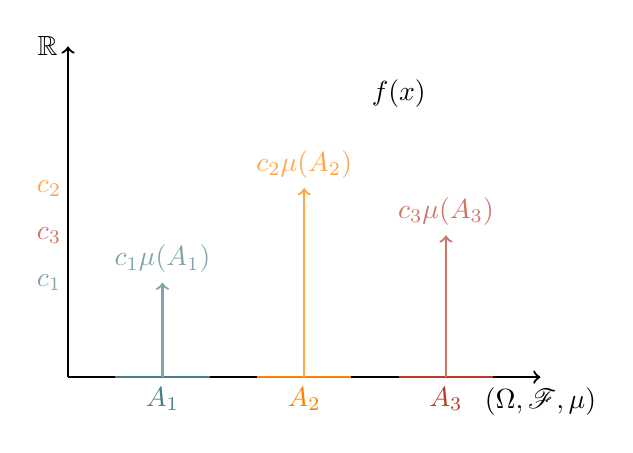
\begin{tikzpicture}[scale=1.2]

% Axes
\draw[thick, ->] (0,0) -- (5,0) node[below] {$(\Omega, \mathscr{F}, \mu)$}; % x-axis
\draw[thick, ->] (0,0) -- (0,3.5) node[left] {$\mathbb{R}$}; % y-axis

% Labels for A1, A2, A3 on x-axis
\draw[green, thick] (0.5,0) -- (1.5,0) node[midway, below] {$A_1$};
\draw[orange, thick] (2,0) -- (3,0) node[midway, below] {$A_2$};
\draw[red, thick] (3.5,0) -- (4.5,0) node[midway, below] {$A_3$};

% Bars representing c_i values
% Bar for A1
\draw[dashed, green!70] (1,0) -- (1,1) node[above, green!70] {$c_1 \mu(A_1)$};
\draw[->, thick, green!70] (1,0) -- (1,1);

% Bar for A2
\draw[dashed, orange!70] (2.5,0) -- (2.5,2) node[above, orange!70] {$c_2 \mu(A_2)$};
\draw[->, thick, orange!70] (2.5,0) -- (2.5,2);

% Bar for A3
\draw[dashed, red!70] (4,0) -- (4,1.5) node[above, red!70] {$c_3 \mu(A_3)$};
\draw[->, thick, red!70] (4,0) -- (4,1.5);

% Labels for c1, c2, c3 on the left
\node[green!70] at (-0.2,1) {$c_1$};
\node[orange!70] at (-0.2,2) {$c_2$};
\node[red!70] at (-0.2,1.5) {$c_3$};

% Function label
\node at (3.5,3) {$f(x)$};

\end{tikzpicture}
	
\end{eg}


\begin{df}{Lebesgue Integral (for Simple Functions)}\\
Define the set 
\[
S^+ := \{ f : \Omega \to \mathbb{R} \mid f\text{ is simple function, } f \geq 0 \}.
\]
For \( f \in S^+ \): define its Lebesgue integral w.r.t. its measure $\mu$ as: 
\[
\int_\Omega f \, d\mu := \sum_{i=1}^n c_i \cdot \mu(A_i), \quad \forall f \in S^+
\]
\end{df}
\textbf{Notation:} 
\[
\int_\Omega f \, d\mu \quad \text{or} \quad \int_\Omega f(x) \, d\mu(x).
\]

\begin{prop}{Lebesgue Integral}
\begin{itemize}
    \item \textbf{Linearity:} \( \int_\Omega (\alpha f + \beta g) \, d\mu = \alpha \int_\Omega f \, d\mu + \beta \int_\Omega g \, d\mu, \quad \forall f, g \in S^+, \alpha, \beta \geq 0. \)
    \item \textbf{Monotonicity:} If \( f \leq g \), then \( \int_\Omega f \, d\mu \leq \int_\Omega g \, d\mu. \)
\end{itemize}	
\end{prop}

\subsection{Lebesgue Integral}
\begin{df}{Lebesgue Integral}
\begin{enumerate}
	\item For any \( f: \Omega \to \mathbb{R} \), define the set $\mathcal{S_f}^+ = \qty{h\in S^+\mid h<f}$.
	\item Compute all Lebesgue integral $I(h)$ according to the previous definition. 
\end{enumerate}
We define 
$$\int_\Omega fd\mu = \sup_{h\in \mathcal{S_f}^+} I(h)$$
And we note that $f$ is $\mu$-integrable (or just integrable if the context if clear) if $\int_\Omega fd\mu <\infty$. 
\end{df}

\subsection{Important results and theorems}

\begin{lem}{Fatou's Lemma}
\noindent Given a measure space $(\Omega, \mathscr{F}, \mu)$ and a sequence of measurable, non-negative functions $\qty{f_n}$ each maps from $(\Omega, \mathscr{F}, \mu) \rightarrow (\R, \mathscr{B}, \cdot)$. Define a function $f \equiv \liminf_{n\to \infty} f_n(x)$, then $f$ is measurable and we have the following inequality: 
$$\int_\Omega f \, d\mu \leq \liminf_{n\to\infty} \int_\Omega f_n \, d\mu$$
\end{lem}

\begin{cor}{Beppo Levi's Monotone Convergence}
Let \((\Omega, \mathscr{F}, \mu)\) be a measure space, and let $\{X_n\}$ be a sequence of non-negative measurable functions defined on $\Omega$. Suppose:
$$0 \leq X_n(\omega) \leq X_{n+1}(\omega) \quad \forall \omega \in \Omega \quad \text{(monotonically increasing sequence of functions)}$$
Define the pointwise limit function:

$$X(\omega) = \lim_{n \to \infty} X_n(\omega), \quad \forall \omega \in \Omega$$
Then:
$$\lim_{n \to \infty} \int_\Omega X_n \, d\mu = \int_\Omega X \, d\mu$$
\end{cor}

\begin{thm}{Lebesgue's Dominated Convergence Theorem}
	\noindent Let $(\Omega, \mathscr{F}, \mu)$ be a measure space, and let $\{f_n\}$ be a sequence of measurable functions mapping from $(\Omega, \mathscr{F}, \mu)$ to $(\mathbb{R}, \mathscr{B})$. Suppose:  
\begin{itemize}
    \item \( f_n \to f \) pointwise almost everywhere on \( \Omega \), and  
    \item there exists an integrable function \( g \colon \Omega \to \mathbb{R} \) such that \( |f_n(\omega)| \leq g(\omega) \) for all \( \omega \in \Omega \) and all \( n \in \mathbb{N} \).
\end{itemize}
	
	Then all $f_n$ and $f$ integrable, and 
	$$\lim_{n\to\infty} \int_\Omega f_n d\mu = \int_\Omega \lim_{n\to\infty} f_n d\mu = \int_\Omega f d\mu$$
\end{thm}


\subsection{Expectation}

\begin{df}{Expectation}
Consider a measure space $(\Omega, \mathscr{F}, P)$ and a random variable $X: \Omega \rightarrow \R$. Its expectation is defined to be a Lebesgue integral
$$\E[X] = \int_\Omega X(\omega) dP(\omega)$$
\end{df}

\begin{cor}{Jensen's Inequality}
If  $X$  is a random variable and  $\phi: \R\rightarrow \R$  is a convex function, then:
$$\phi(\mathbb{E}[X]) \leq \mathbb{E}[\phi(X)]$$
Special Case: For $\phi(x) = |x|$, we obtain:
$$\abs{\mathbb{E}[X]} \leq \mathbb{E}\qty[\abs{X}]$$
Intuition: The expectation of a convex function applied to  X  is at least as large as applying the function to the expectation of  X . Convexity “pulls the curve upwards,” leading to this inequality.
\end{cor}

\begin{cor}{Markov's Inequality}
For a non-negative random variable $X$ and any $\alpha > 0$. 

$$P(|X| > \alpha) \leq \frac{\mathbb{E}[|X|]}{\alpha}$$
Intuition: The probability that $X$ exceeds some threshold $\alpha$ is bounded by the ratio of its expected value to  $\alpha$. It provides an upper bound on tail probabilities.
\end{cor}



\subsection{Chebyshev's Inequality}
\textbf{Statement:} For $f: \R^d \to \R, f\geq 0, \alpha \in \R$, we have $m(\qty{f\geq \alpha}) <\frac{1}{\alpha}\int f$. \\

\begin{prf}
By monotonicity of integral, 
$$\int f\geq \int_{\qty{f\geq \alpha}} f$$
Also observe that 
$$\int_{\qty{f\geq \alpha}} f \geq \alpha\cdot m(\qty{f\geq \alpha})\quad \text{Since }f\geq \alpha \text{ a.e. on the set}$$
Associating the two inequalities: 
$$\frac{1}{\alpha} \int f\geq m(\qty{f\geq \alpha})$$

\end{prf}

\textbf{Two immediate lemmas follow: }
\subsubsection{Lemma 1}
\textbf{Statement:}For $f:\R^d\to [0, \infty]$, if $\int f<\infty$, then $f<\infty$ a.e.\\

\begin{prf}
	Fix any $n\in \N$, by Chebyshev's inequality, 
	$$m\qty{f\geq n} < \frac{1}{n} \underbrace{\int f}_{<\infty}$$
	And the sequence of sets: $\qty{f\geq n}_{n\in \N}$ are nested and $ \qty{f\geq n}\searrow \qty{f>\infty}$. Therefore by continuity of measure: 
	\begin{align*}
		\lim_{n\to\infty} m(\qty{f\geq n}) &\leq \lim_{n\to\infty} \frac{1}{n}\int f\\
		m(\qty{f>\infty}) &\leq 0\\
	\end{align*}
	Therefore, $f$ goes to infinity on a set of measure 0, which is equivalent as $f$ is finite almost everywhere. 
	
	
\end{prf}

\subsubsection{Lemma 2}
\textbf{Statement:} For $f: \R^d \to [0, \infty]$, if $\int f = 0$, then $f=0$ a.e.\\

\begin{prf}
Similarly, fixing $n\in \N$, we have by Chebyshev's inequality: 
\begin{align*}
	m(\qty{f\geq 1/n}) &< n\int f = 0
\end{align*}
Observe that the sequence of sets $\qty{f\geq 1/n}_{n\in \N}$ is an increasing sequence of sets such that $\qty{f\geq 1/n} \nearrow \qty{f>0}$. Therefore by continuity of measure: 
\begin{align*}
	\lim_{n\to\infty} m\qty(\qty{f\geq 1/n}) &\leq n\int f\\
	 m\qty(\qty{f>0}) &\leq 0
\end{align*}

Therefore, the set on which $f$ is strictly larger than 0 has measure 0. This is equivalent as $f = 0$ almost everywhere. 

\end{prf}

\subsection{Fatou's Lemma}
\textbf{Statement} Given a sequence of functions $\qty{f_n}_{n\in \N}$,  $f_n\geq 0 \ \forall n$. If $f_n\to f$ almost everywhere. Then $\int f \leq \liminf_{n} \int f_n$. \\

\begin{prf}
Same practice that we can always remove the subset from the domain on which 	$f_n$ does not converge to $f$, therefore making $f_n\to f$ pointwise everywhere.\\

Consider a function $g$ bounded with finite support: $m(\mathrm{supp}(g))<\infty$, and $0\leq g\leq f$. Reminder that the construction of $g$ is qualified for the bounded convergence theorem. \\

Then we set $g_n\equiv \min\qty{g, f_n}$. Given $g<f$ and $f_n\to f$, we know that $g_n\to g$. \\

By bounded convergence theorem, 
$$\int g = \lim_{n\to\infty} g_n$$
By monotonicity: 
$$\forall n, \ g_n \leq f_n \Rightarrow \int g_n \leq \int f_n$$
We take the limit inferior on both ends (since we don't know yet if the limits exist): 
\begin{align*}
	\underbrace{\liminf_{n}\int g_n}_{=\lim_n \int g_n} &\leq \liminf_{n}\int f_n\\
	\int g &\leq \liminf_{n}\int f_n \quad \forall g\leq f\\
	\underbrace{\sup_{g\leq f}\int g}_{\text{definition of }\int f} &\leq \liminf_{n}\int f_n\\
	\int f &\leq \liminf_{n}\int f_n 
\end{align*}

\end{prf}

\subsection{Monotone Convergence Theorem}
\begin{prf}

\textbf{Statement} For a sequence of function $f_k: \R^d \to \R, f_k\geq 0.$ If $f_k$ monotonically converges to some limit function $f$, then 
$$\lim_{k\to\infty}\int f_k = \int f$$
By monotonicity of integral, $\qty{f_k}$ being a monotone sequence implies that $\qty{\int f_k}$ is also a monotone sequence bounded by $\int f$. Therefore, $\lim_{k\to\infty} \int f_k$ exists and is smaller than $\int f$. \\

The other side of the inequality is given by Fatou's lemma: 
$$\int f \leq \liminf_k \int f_k = \lim_k \int f_k$$
Therefore, we have $\int f = \lim_k \int f_k$. 

\end{prf}
\subsection{Dominated Convergence Theorem}
\textbf{Statement} For a sequence of functions $f_k: \R^d \to \R$ and $f_k\to f$ a.e.. If $\exists g$ integrable such that $\abs{f_k}\leq g \ \forall k$, then $\lim_{k\to\infty} \int \abs{f_k-f} = 0$. \\

\begin{prf}
We focus on the function $2g-\abs{f_k-f}$, note that $\abs{f_k}\leq g$ implies that $\abs{f}\leq g$, and 
$$\abs{f_k - f}\leq \abs{f_k} + \abs{f} \leq 2g$$
Therefore $2g-\abs{f_k-f}\geq 0$. \\

By Fatou's lemma,
\begin{align*}
	\liminf_{k} \int 2g - \abs{f_k-f} &\geq \int 2g - \lim_k \abs{f_k-f} = \int 2g\\
	\int 2g - \liminf_{k}\int \abs{f_k-f} &\geq \int 2g\\
	\limsup_k \int \abs{f_k-f} - \int 2g &\leq -\int 2g\\
	\limsup_k \int \abs{f_k-f}&\leq 0
\end{align*}
Given that $\int \abs{f_k-f}\geq 0$ by definition, we conclude that $\lim_{k\to\infty}\int \abs{f_k-f}= 0$.\\

Remark: This conclusion, in particular, states that $\int f_k\to \int f$.  

\end{prf}
\subsection{Other Propositions to Integrability}
\subsubsection{Proposition I}
\textbf{Statement} For $f: \R^d\to \R$ integrable, then $\forall \ep>0, \exists E \subset \R^d, m(E)<\infty, and \int_E \abs{f}<\ep$. \\

\begin{prf}
We define $E_N \equiv \qty{\abs{x}<N}$. \\
Observe the sequence of functions $\abs{f}\cdot \chi_{E_N}$ are measurable and converges pointwise monotonically to $\abs{f}$. We can then apply monotonic convergence theorem to conclude that
\begin{align*}
	\lim_{N\to\infty}\int\abs{f}\chi_{E_N} &= \int\abs{f}
\end{align*}
Then by this convergence, $\exists N$ such that the difference $E\equiv \R^d\backslash E_N$ such that
$$\int_{E} \abs{f} =\int_{\R^d}\abs{f} - \int_{E_n}\abs{f} <\epsilon$$


Remark: \textcolor{teal}{The setup $\abs{f}\chi_{E_N}$ is also dominated by $f$ so DCT also works for this setup.}

\end{prf}

\subsubsection{Proposition II: Absolute Continuity}
\textbf{Statement} For $f: \R^d\to \R$ integrable, then $\forall \ep>0, \exists \delta>0$ such that $\forall E\subset \R^d$ measurable with $m(E)<\delta$, $\int_E \abs{f}<\ep$.\\ 

\begin{prf}
We will prove this by contradiction: Suppose this is not true. \\

Then $\exists \ep>0$ such that we cannot find a $\delta$, that is, $\forall n$, there are some exceptions on some sets $E_n$, we set it up by letting $m(E_n) <1/2^n$ and $\int_E \abs{f}\geq \ep$. \\

Then notice that the measure of $E_n$ is designed to be summable and the infinite sum converges - then we have Borel-Cantelli Lemma: 
$$\sum_n m(E_n) < \infty \Rightarrow m\qty(\limsup_n E_n) = 0$$

\textcolor{teal}{Recall $\limsup_n E_n = \cap_{n\in\N}\cup_{k\geq n} E_n$}\\

We define the limsup set to be $E$. Since $m(E) = 0$, $\int_E \abs{f} = 0$. Observe the set of union $\cup_{k\geq n}E_n$, the sequence of functions $\abs{f}\cdot\chi_{\bigcup_{k\geq n} E_n}$ are all bounded above by $\abs{f}$, then by DCT: 
\begin{align*}
	\lim_{n\to\infty}\int_{\bigcup_{k\geq n} E_n} \abs{f} &= \int_E\abs{f} = 0
\end{align*}
However, $\int_{E_n} \abs{f}\geq \ep > 0 \ \forall n$. This is a contradiction to the previous conclusion that the limit of the integral goes to 0. We therefore proved the proposition of absolute continuity.



\newpage
\section{Moment Generating Functions and Characteristic Functions}

\subsection{Moment Generating Functions}

\begin{df}{MGF}\\
Given $X: \Omega \to \mathbb{I} \subset \mathbb{R}$ with a measure space $(\Omega, \mathscr{F}, P)$ where $|\mathbb{I}|$ is countable, the \textbf{Moment Generating Function (MGF)} $m_X(t)$ is defined as:
$$m_X(t) \equiv \mathbb{E}[e^{tX}]$$
\end{df}

\begin{rmk}{}
It is possible for $m_X(t) = \infty$. In fact, very few random variables have MGF. 
\end{rmk}

\begin{rmk}{}
If:
\begin{enumerate}
    \item There exists $t \neq 0$ such that $m_X(t)$ is finite for $t \in (-\epsilon, \epsilon)$ for some small $\epsilon$.
    \item $m_X(t)$ is differentiable $k$ times at $t = 0$.
\end{enumerate}
Then:
\[
\mathbb{E}[X^k] = \frac{\partial^k m_X(t)}{\partial t^k} \bigg|_{t=0}.
\]
\end{rmk}


\subsection{Characteristic Function:}

\begin{df}{Characteristic Function}\\
The \textbf{Characteristic Function (CF)} $\phi_X: \R\rightarrow \mathbb{C}$, of a random variable $X$ is defined as:
\[
\phi_X(t) = \mathbb{E}[e^{itX}], \quad t \in \mathbb{R}.
\]
It is the complex analogue of the MGF
\end{df}
\begin{prop}{Properties of CF}
\begin{itemize}
    \item $\exp(itX)$ is bounded by the unit circle since $\lvert e^{itX} \rvert = \cos(tX) + i\sin(tX) \leq 1$ 
    \item The characteristic function $\phi_X(t)$ is always well-defined.
    \item Note that if $X$ is multidimensional, $tX$ is defined by the inner product.
\end{itemize}	
\end{prop}

\begin{thm}{}
If $\mathbb{E}[|X|^k] < \infty$, then $\exists \varphi^{(k)}(t)$ for $k = 1, \dots, n \ \forall t\in \R$, and  
\[
\frac{\partial^k \phi_X(t)}{\partial t^k} \bigg|_{t=0} = i^k \mathbb{E}[X^k].
\]
This is true by Lebesgue's DCT, given the characteristic function is always bounded by the unit circle therefore the limit (from differentiation) and the integral sign are always interchangeable. 
\end{thm}


\subsection{Convergence in Distribution:}


\begin{df}{Convergence in Distribution}\\
A sequence of random variables $X_n$ converges in distribution to $X$ (denoted $X_n \xrightarrow{d} X$) if:
\[
\forall t \in \mathbb{R}, \quad \phi_{X_n}(t) \to \phi_X(t).
\]
\noindent Where $\phi$ is the characteristic function of the push-forward measure.	
\end{df}
\begin{rmk}{}
	Note that convergence in distribution happens in the codomain, whereas the aforementioned almost surely convergence and convergence in probability happen in the domain (latent space $\Omega$). 
\end{rmk}



\begin{prop}{TFAE}
\begin{enumerate}
    \item $\forall t \in \mathbb{R}, \ \phi_{X_n}(t) \to \phi_X(t)$.
    \item $\forall \varphi \in \mathscr{C}_b(\mathbb{R}), \ \mathbb{E}[\varphi(X_n)] \to \mathbb{E}[\varphi(X)]$.
    \item The cumulative distribution functions converge at all points of continuity:
    \[
    F_n(x) \to F(x).
    \]
\end{enumerate}	
\end{prop}

\begin{thm}{Levy's Theorem}
	 A sequence $X_j$ of n-variate random variables converges in distribution to random variable $X$ if and only if the sequence $\varphi_{X_j}$ converges pointwise to a function $\varphi$ which is continuous at the origin. Where $\varphi$  is the characteristic function of the limit $X$.\\
	 
	 The definition $\Leftrightarrow$ the first equivalent condition.  
\end{thm}


\noindent \textbf{Note:} Convergence in distribution $X_n \xrightarrow{d} X$ is weaker than convergence in probability or almost sure convergence:
\[
X_n \xrightarrow{a.s.} X \implies X_n \xrightarrow{P} X \implies X_n \xrightarrow{d} X.
\]

\subsection{Characterization of a Distribution:}
\begin{thm}{Characterization of a Distribution}
Two distributions $P_X$ and $P_Y$ are equal if and only if their characteristic functions are equal:
\[
P_X = P_Y \iff \phi_X(t) = \phi_Y(t) \quad \forall t \in \mathbb{R}.
\]
* Knowing the characteristic function knows all the moments, knowing all the moments knows the distribution. 
\end{thm}


\subsection{Application: De-Convolution}
\noindent If $X_1$ and $X_2$ are independent random variables:
\[
\phi_{X_1 + X_2}(t) = \phi_{X_1}(t) \cdot \phi_{X_2}(t).
\]
Given $X_n = X + V$, if we know $\phi_{X_n}$ and $\phi_V$, we can recover the distribution of $X$:
\[
P_X = \frac{\phi_{X_n}}{\phi_V}.
\]


\newpage
\section{The General Prediction Problem}
\subsection{Hilbert Space}
Note that Hilbert space and functional analysis is not the focus of this note. Just a brief introduction here. 

\begin{df}{Hilbert Space}\\
A \textbf{Hilbert space} $\mathscr{H}$ is a vector space equipped with an inner product $\langle \cdot, \cdot \rangle$, which induces a norm $\| x \| = \sqrt{\langle x, x \rangle}$, such that $\mathscr{H}$ is:
\begin{itemize}
    \item \textbf{Complete:} Every Cauchy sequence in $\mathscr{H}$ converges to a limit within $\mathscr{H}$.
    \item \textbf{Linear:} Closed under vector addition and scalar multiplication. Note that the \textbf{function space} is linear, not the functions themselves necessarily. 
    \item \textbf{Inner Product Space:} Equipped with an inner product $\langle \cdot, \cdot \rangle$ satisfying symmetry, linearity, and positivity.
\end{itemize}
Note that if we define an inner product $\langle f, g \rangle$ in squared integrable functions as 
$$\langle f, g \rangle = \int_\Omega f\cdot g\, d\mu$$
Then the space of squared integrable functions, denoted by $L^2(\mu)$, is a Hilbert space. 
\end{df}


\subsection{General Prediction Problem}
\begin{itemize}
    \item Goal: Predict a real-valued random variable $Y$ based on random covariates $X \in \mathbb{R}^d$ using a function $h(X)$.
    \item Assumptions: The prediction function $h$ belongs to a linear vector space $\mathcal{V}$. 
    \item Maintained Assumptions: $h, Y \in \mathcal{V}$ if $\lambda g + \mu h \in \mathcal{V}$ and $1 \in \mathcal{V}$.
\end{itemize}
We have the following optimisation problem w.r.t. the \textbf{mean square error}: 
\begin{align*}
\min_{h \in \mathcal{V}} \mathbb{E} \big[ (Y - h(X))^2 \big].
\end{align*}
The choice of mean square error as the objective function for this minimization problem is a convenient discretion since it induces a Hilbert space. 

\begin{thm}{Conditional Expectation}
\textit{The function $h^*(X)$ that minimizes the MSE satisfies:}
\[
h^*(X) = \underset{h \in \mathscr{H}}{\arg \min} \, \mathbb{E} \big[ (Y - h(X))^2 \big]
\]
Is the conditional expectation function (to be defined later)
$$h^*(X) = \E[Y|X]$$
Characterized by 
$$Y = \E[Y|X] + \ep$$
With
\begin{itemize}
    \item $\mathbb{E}[\varepsilon] = 0$ (zero mean),
    \item $\text{Cov}(\varepsilon, h(X)) = 0, \, \forall h \in \mathscr{H}$.
\end{itemize}	
\end{thm}

\begin{rmk}
MSE can be decomposed as variance + bias:
\[
\mathbb{E} \big[ (Y - h(X))^2 \big] = \underbrace{\text{Var}[Y - h(X)]}_{\text{Variance}} + \big( \underbrace{\mathbb{E}[Y] - \mathbb{E}[h(X)]}_{\text{Bias}} \big)^2.
\]
Since $h\in \mathscr{H}$ contains the unit element therefore all constant functions, we can set the bias equal to zero without affecting the variance to a certain extent. 
\end{rmk}

\subsection{Optimality Conditions}
\begin{itemize}
    \item \textbf{Necessary condition for optimality:} $h^*(X)$ is optimal if:
    \[
    \text{Cov}(Y - h^*(X), h(X)) = 0 \quad \forall h \in \mathcal{V}.
    \]
    \item \textbf{Sufficient condition for optimality:}
    \[
    \mathbb{E} \big[ (Y - h^*(X)) h(X) \big] = 0.
    \]
\end{itemize}

\begin{thm}{}
\begin{itemize}
    \item \textit{If $h^*(X) \in \mathscr{H}$, it is unique almost surely.}
    \item \textit{If $\mathscr{H}$ is a closed subspace of $L^2(P)$, then $h^*(X)$ exists and is optimal.}
\end{itemize}	
\end{thm}


\begin{eg}{Affine Regression}\\
Let $\mathcal{V}$ be the vector space spanned by $1, X_1, \ldots, X_d$. Then:
\[
h^*(X) = a + b^\top X, \quad \text{where} \quad
\begin{cases}
    a = \mathbb{E}[Y] - b^\top \mathbb{E}[X], \\
    b = \text{Var}(X)^{-1} \text{Cov}(X, Y).
\end{cases}
\]
\textit{Solution:} 
\[
\hat{\beta} = (X^\top X)^{-1} X^\top Y.
\]
And 
\[
X\hat{\beta} = \underbrace{X(X^\top X)^{-1} X^\top}_{\equiv P \text{ Projection matrix}} Y.
\]
\end{eg}


\subsection*{Projection Interpretation}
\[
h^*(X) = \mathbb{E}[Y | X]
\]
is the \textit{unique argument} minimizing the MSE. The solution can be interpreted as a projection of $Y$ onto $\mathscr{H}$, a subspace of $L^2(\mathbb{P})$, which is a Hilbert space.

\subsection{Properties}
There is \textbf{no} full closed form for \(\mathbb{E}[Y \mid X]\). All we know is:
\begin{itemize}
    \item \(\mathbb{E}[Y \mid X]\) is the only function in \(L^2(P)\) of \(X\) such that:
    \[
    \mathbb{E}[Yh(X)] = \mathbb{E}[\mathbb{E}[Y \mid X]h(X)] \quad \forall h(X) \in L^2(P).
    \]
    \item \(\operatorname{cov}(Y, h(X)) \iff \operatorname{cov}(Y, h(X)) = 0\), so anything outside the \(L^2(P)\) differs by an orthogonal function \(\implies\) doesn't matter.
\end{itemize}


\subsubsection{Discrete Case}

\[
\mathbb{E}[Y \mid X = x]: \mathbb{R} \to \mathbb{R}, \ \text{thus depends on } x.
\]
\begin{clm}
\[
\mathbb{E}[Y \mid X = x] = \sum_y y \cdot P_{Y|X}(Y=y|X=x)\equiv \psi(x)
\]
where
\[
P_{Y \mid X}(Y \mid X = x) = \frac{P(\{Y = y\} \cap \{X = x\})}{P(X = x)}.
\]
\end{clm}

\newpage
\section{The Gaussian Distribution}


\newpage
\section{Introduction to Asymptotic Theory}

%%%%%%%%%%%%%%%%%%%%%%%%%% APPENDIX %%%%%%%%%%%%%%%%%%%%%%
\newpage
\appendix
\section{Some Proofs}
\subsection{Discrete Probability Measure}
\subsubsection{Boole's Inequality}
\label{proof: boole}
\textbf{Statement:}
$P\left(\bigcup_{n=1}^\infty A_n\right)\leq\sum_{n=1}^\infty P(A_n)$

\begin{prf*}
We first construct a sequence of disjoint sets $B_n$ that each set in the sequence is defined the following: 
$$B_1 = A_1, B_2 = A_2 \backslash A_1, B_3 = A_3\backslash (A_2\cup A_1), \dots B_n = A_n \backslash \qty(\bigcup_{i=1}^{n-1}A_i)$$ 
\begin{clm}
All $B_n$ disjoint.
\end{clm}

To show this, fix $m, k\in \N$ and observe $B_m$ and $B_k$. Without loss of generality, suppose that $m<k$. Fix $b\in B_m$, then $b\in A_m$. We can also write $B_k = A_k \backslash \qty(\bigcup_{i=1}^{k-1}A_i) = A_k \backslash \qty(\bigcup_{i=1}^{m-1}A_i \cup A_m \cup \bigcup_{i=m+1}^{k-1}A_i)$ which has $A_m$ cut out in the second part. Therefore, $b\notin B_k$. \\

Similarly, fix $c\in B_k$, then $c\notin A_m$, but $\forall b\in B_m, b\in A_m$. So $c\notin B_m$. We have shown that all $B_n$ disjoint. \\

Therefore, for any two $B_m, B_k$, $B_m\cap B_k = \varnothing$. We have all $B_i$ disjoint. 

\begin{clm} 
$\bigcup_{n=1}^\infty A_n = \bigcup_{n=1}^\infty B_n$.	
\end{clm}

To show this, $\bigcup_{n=1}^\infty B_n \subseteq \bigcup_{n=1}^\infty A_n$ is trivial as all $B_n \subset A_n$ by construction. We now need to show the converse is true as well. Fix $a\in \bigcup_{n=1}^\infty A_n$, then $\exists$ some $m$ such that $a\in A_m$, then we have two scenario: \\

\noindent \textbf{Scenario 1: } $a\in A_m \backslash \qty(\bigcup_{i=1}^{m-1}A_i)$\\
Then $a\in B_m$ which implies $a\in \bigcup_{n=1}^\infty B_n$, we have $\bigcup_{n=1}^\infty A_n \subseteq \bigcup_{n=1}^\infty B_n$. \\



\noindent \textbf{Scenario 2: } $a\notin A_m \backslash \qty(\bigcup_{i=1}^{m-1}A_i)$.\\
This implies that $a\in \qty(\bigcup_{i=1}^{m-1}A_i)$, then $\exists k<m$ such that $a\in A_k$. We could again break it into the above two scenarios by replacing $m$ with the new $k$. This process will not be infinite as falling into scenario 2 will give us a new index that is strictly smaller than the previous one. Since $n\in \N^+$, $a$ has to belong to some $A_l\backslash \qty(\bigcup_{i=1}^{l-1}A_i) = B_l$. Then $a\in \bigcup_{n=1}^\infty B_n$. We have shown that $\bigcup_{n=1}^\infty A_n \subseteq \bigcup_{n=1}^\infty B_n$, therefore  $\bigcup_{n=1}^\infty A_n = \bigcup_{n=1}^\infty B_n$. \\

Since $B_n \subseteq A_n \ \forall n$, we have the monotonicity of the measures: 
\begin{align*}
	P(B_n) &\leq P(A_n)\\
	\sum_{n=1}^\infty P(B_n) &\leq \sum_{n=1}^\infty P(A_n)
\end{align*} 
By Kolmogorov axiom 3, we have $P\qty(\bigcup_{n=1}^\infty B_n) =  \sum_{n=1}^\infty P(B_n) \ \forall B_n$ disjoint, we have: 
\begin{align*}
	P\qty(\bigcup_{n=1}^\infty B_n) =  \sum_{n=1}^\infty P(B_n) &\leq \sum_{n=1}^\infty P(A_n)
\end{align*} 
By above claim 2, we have $\bigcup_{n=1}^\infty A_n = \bigcup_{n=1}^\infty B_n$, then
\begin{align*}
	P\qty(\bigcup_{n=1}^\infty A_n) = P\qty(\bigcup_{n=1}^\infty B_n) =  \sum_{n=1}^\infty P(B_n) &\leq \sum_{n=1}^\infty P(A_n)\\
	P\qty(\bigcup_{n=1}^\infty A_n)  &\leq \sum_{n=1}^\infty P(A_n)
\end{align*} 
\end{prf*}




\subsubsection{Bonferroni's Inequality}
\label{proof: bonferroni}
\textbf{Statement: }for fixed $n\in \N$,  $P(\bigcap_{i=1}^nA_i)\geq \sum_{i=1}^n P(A_i)-n+1$.

\begin{prf*}
	Given the left hand side
	\begin{align*}
		P\qty(\bigcap_{i=1}^nA_i) &= 1-P\qty(\overline{\bigcap_{i=1}^nA_i})\\
		&= 1 - P\qty(\bigcup_{i=1}^n \overline{A_i}) \quad \text{By De Morgan's law}\\
		&\geq 1-\sum_i P(\overline{A_i}) \quad\text{By Boole's inequality}\\
		&\geq 1 - \sum_i (1-P(A_i))\\
		&\geq 1 - n + \sum_i P(A_i)
	\end{align*}
\end{prf*}


\subsection{Stochastic Convergence}

\subsubsection{Equivalent Conditions on almost sure convergence}

\subsubsection{Borel-Cantelli Lemma}

\subsubsection{Convergence almost surely implies convergence in probability}
\label{proof: a.s.convergence implies convergence in prob}
\begin{prf*}
	For simplicity, assuming the random variable $X_n\rightarrow 0$. Then by definition, 
	$$P\left( \limsup_{n \to \infty} \{|X_n| > \epsilon\} \right) = 0$$
	Then by Borel-Cantelli's lemma, almost sure convergence implies the convergence of the infinite sum of probabilities: 
	$$\sum_{n=1}^\infty P\qty[\{|X_n| > \epsilon\}] < \infty$$
	Above implies that each term for sufficiently large $n$ must converge to 0,	
	$$\lim_{n\to\infty} P\qty[\{|X_n| > \epsilon\}] = 0$$
	We have $X_n$ converges to 0 in probability. 
\end{prf*}

\subsection{Non-existence of measure}
\label{proof: non-existence}
\begin{prf*}\\
\textbf{Construction:}\\
Define the interval \( I = (0, 1] \) with an equivalence relation \( x \sim y \) if \( x - y \in \mathbb{Q} \). That is:
\[
[x] = \{x + r \mid r \in \mathbb{Q}, x \in I\}.
\]
This partitions \( I \) into disjoint sets.

\noindent Pick \( A \subseteq I \) with:
\begin{enumerate}
    \item[i)] \(\forall x, y \in A, \, x \sim y \implies x = y\),
    \item[ii)] For each \( x \in I \), if \( x \in [x] \) for some \( x \), then \( x + r \in A \), where \( A_i = x + A \).
\end{enumerate}

\begin{clm}Disjointness of Shifts: If \( A_n = A + r_n \), where \( r_n \) is an enumeration of \( \mathbb{Q} \cap (-1, 1) \), then:
\[
A_n \cap A_m = \varnothing \quad \text{for } n \neq m.
\]
\end{clm}

\noindent Suppose \( x \in A_n \cap A_m \). Then:
\[
x \in A + r_n \quad \text{and} \quad x \in A + r_m.
\]
This implies:
\[
x = a + r_n \quad \text{and} \quad x = a' + r_m \implies r_n - r_m \in \mathbb{Q}.
\]
By the construction of \( A \), this forces \( r_n = r_m \), which is a contradiction. Thus \( A_n \cap A_m = \varnothing \) for \( n \neq m \).

\begin{clm}[Covering of \((0, 1]\)]
\[
(0, 1] \subseteq \bigcup_{n \in \mathbb{N}} A_n \subseteq (-1, 2).
\]
\end{clm}

\begin{enumerate}
    \item[(i)] The first inclusion is given since all \( A_n \) serve as a partition of \((0, 1]\),
    \item[(ii)] By construction, for all \( x \in \bigcup_{n \in \mathbb{N}} A_n \), there exists \( i \in \mathbb{N} \) such that \( x \in A + r_i \). Since \( A \subseteq (0, 1] \), we conclude:
    \[
    x \in \mathbb{R} \cap (-1, 2).
    \]
\end{enumerate}

By property (ii), \( \mu(x + A) = \mu(A) \) for all \( x \in \mathbb{R} \). By Claim 2:
\[
\mu((0, 1]) \leq \mu\left(\bigcup_{n \in \mathbb{N}} A_n\right) \leq \mu((-1, 2)).
\]
We know \(\mu((0, 1]) = C < \infty\). Then:
\[
\mu((-1, 2)) = \mu((-1, 0]) + \mu((0, 1]) + \mu((1, 2]) = 3C.
\]
Thus:
\[
C \leq \sum_{n=1}^\infty \mu(A_n) \leq 3C.
\]
If \( \mu(A) > 0 \), this leads to a contradiction such that an item bounded above by a finite value $3C$ diverges to infinity. Therefore:
\[
\mu(A) = 0.
\]

\end{prf*}


\subsection{Proving Measurability}
\label{proof: measurability}

\begin{prf}
We prove this result in two directions.

Let \(X: \Omega \to \mathbb{R}^d\) be a function. Then:
\[
\sigma(X) = \sigma\left(X^{-1}(\mathcal{L})\right),
\]
where \(\mathcal{L}\) is a generator of the Borel \(\sigma\)-algebra \(\mathscr{B}^d\).

\paragraph{1. Forward Direction:}  
We show that:
\[
X^{-1}(\mathcal{L}) \subseteq \sigma(X).
\]
\begin{itemize}
    \item By the definition of the \(\sigma\)-algebra \(\sigma(X)\), it contains all preimages of measurable sets under \(X\).
    \item Specifically, for all \(A \in \mathscr{B}^d\), we know that \(X^{-1}(A)\) is measurable.
    \item Since \(\mathcal{L}\) is a generator of \(\mathscr{B}^d\), any set in \(\mathscr{B}^d\) can be written as a countable combination (union, intersection, complement) of sets in \(\mathcal{L}\).
    \item Therefore, \(X^{-1}(\mathcal{L}) \subseteq \sigma(X)\).
\end{itemize}

\paragraph{2. Reverse Direction:}  
We show that:
\[
\sigma(X) \subseteq \sigma\left(X^{-1}(\mathcal{L})\right).
\]
\begin{itemize}
    \item Define \(\mathscr{F}_X = \{ B \in \mathscr{B}^d \mid X^{-1}(B) \in \sigma(X^{-1}(\mathcal{L}))\}\subseteq \mathscr{B}^d\).
    \item We will skip proving the following two points:
    \begin{enumerate}
        \item \(\mathscr{F}_X\) is a \(\sigma\)-algebra.
        \item \(\mathcal{L} \subseteq \mathscr{F}_X\) (principle of good sets).
    \end{enumerate}
    \item Since \(\mathscr{B}^d\) is the smallest \(\sigma\)-algebra containing \(\mathcal{L}\), we conclude that:
    \[
    \mathscr{B}^d \subseteq \mathscr{F}_X.
    \]
    \item Therefore, for all \(A \in \mathscr{B}^d\), \(X^{-1}(A) \in \sigma(X^{-1}(\mathcal{L}))\).
\end{itemize}

\paragraph{Conclusion:}  
Combining both directions, we obtain:
\[
\sigma(X) = \sigma\left(X^{-1}(\mathcal{L})\right).
\]
	
\end{prf}


\section{Poisson Distribution from Binomial distribution}
\begin{thm}{}
Let $\qty{X_n}_{n\in \N^+}$ be a sequence of random variables defined on a probability space $(\Omega, \mathcal{B}, P)$ and suppose that
$$X_n\sim \mathrm{Binom}\qty(n, \frac{\lambda}{n})$$
Then $X_n\xrightarrow{d} X$ such that $X\sim \mathrm{Poisson}(\lambda)$. 
\end{thm}

\begin{prf*}
To show the convergence in distribution, we need to show that the probability densities converge to a limit density, that is, 
$$\lim_{n\to\infty} P(X_n=k) = P(X=k) = e^{-\lambda}\frac{\lambda^{k}}{k!}$$
Fix $k\in \N^+$, given each $X_n\sim\mathrm{Binom}\qty(n, \frac{\lambda}{n})$, we have
\begin{align*}
	\lim_{n\to\infty} P(X_n = k) &= \lim_{n\to\infty}\binom{n}{k} \qty(\frac{\lambda}{n})^{k}\qty(1-\frac{\lambda}{n})^{n-k}\\
	&= \lim_{n\to\infty}\frac{n!}{k!(n-k)!}\qty(\frac{\lambda}{n})^{k}\qty(1-\frac{\lambda}{n})^{n}\qty(1-\frac{\lambda}{n})^{-k} \quad \text{definition of binomial coefficient}\\
	&= \underbrace{\frac{\lambda^k}{k!}}_{\textcolor{blue}{\text{Poisson-ish}}}\lim_{n\to\infty}\frac{n!}{(n-k)!}\qty(1-\frac{\lambda}{n})^{n}\frac{1}{n^k\qty(1-\frac{\lambda}{n})^k} \quad \text{grouping terms and factoring}\\
	&= \frac{\lambda^k}{k!}\lim_{n\to\infty}\qty{n(n-1)\cdots(n-k+1)}\qty(1-\frac{\lambda}{n})^{n}\frac{1}{(n-\lambda)^k}\\
	&= \frac{\lambda^k}{k!}\lim_{n\to\infty}\underbrace{\frac{\qty{n(n-1)\cdots(n-k+1)}}{(n-\lambda)^k}}_{(1)}\underbrace{\qty(1-\frac{\lambda}{n})^{n}}_{\rightarrow e^{-\lambda} \text{ by def}}
\end{align*}
Notice that term $(1)$ expands to: 
\begin{align*}
	\lim_{n\to\infty} \frac{n(n-1)\cdots(n-k+1)}{(n-\lambda)^k} &= \lim_{n\to\infty} \frac{n^k}{n^k \qty(1 - \frac{\lambda}{n})^k} \prod_{j=0}^{k-1} \qty(1 - \frac{j}{n})\\
	&= \lim_{n\to\infty} \qty(1-\frac{\lambda}{n})^{-k}\cdot \prod_{j=0}^{k-1} \qty(1 - \frac{j}{n})\\
	&= 1
\end{align*}
The first term and each term in the product go to 1. Therefore, $\lim_{n\to\infty}(1) = 1$.\\

\noindent We have shown that $\exists X$ s.t. $\lim_{n\to\infty} X_n = X$ and $X\sim \mathrm{Poisson}(\lambda)$. 
\end{prf*}


A more standard approach in proving weak convergence (convergence in distribution) is to look at the pointwise convergence in the characteristic functions. For \(X_n \sim \mathrm{Binomial}\qty(n, \frac{\lambda}{n})\),
\begin{clm*}
$$\varphi_{X_n}(t) = \mathbb{E}\bigl[e^{\,i\,t\,X_n}\bigr] = \qty(1 - \frac{\lambda}{n} + \frac{\lambda}{n}\,e^{\,i\,t})^{n}$$
\end{clm*}
%
%\noindent To show this: 
%\begin{align*}
%	\varphi_{X_n}(t) &= \mathbb{E}\bigl[e^{\,i\,t\,X_n}\bigr]\\
%	&= \sum_{k=0}^n e^{itk} \cdot P(X_n = k)\\
%	&= \sum_{k=0}^n \binom{n}{k} \qty(e^{it}\frac{\lambda}{n})^k \qty(1-\frac{\lambda}{n})^{n-k}
%\end{align*}
%According to the binomial theorem, for $x, y\in \R, (x+y)^n = \sum_{k=0}^n \binom{n}{k} x^ky^{n-k}$. In this case, let $x \equiv e^{\,i\,t}\frac{\lambda}{n}$ and $y = \qty(1-\frac{\lambda}{n})$, we have the above expression simplified into 
%$$\varphi_{X_n}(t) = \qty( e^{\,i\,t}\frac{\lambda}{n} + 1 - \frac{\lambda}{n})^n$$
\noindent Then the convergence becomes more apparent as
\begin{align*}
	\lim_{n\to\infty} \varphi_{X_n}(t) &= \lim_{n\to\infty} \qty( 1 - \frac{\lambda}{n} + \frac{\lambda}{n}\,e^{\,i\,t})^{n}\\
	&= \lim_{n\to\infty} \left(1 + \frac{\lambda\qty(e^{\,i\,t}-1)}{n}\right)^{n}\\
	&= \exp{\lambda\qty(e^{\,i\,t}-1)}
\end{align*}
The result is precisely the characteristic function of a Poisson-distributed random variable. \\

%Similarly, to show this, suppose that we have a random variable $Y\sim \mathrm{Poisson}(\lambda)$, then by definition, we have its characteristic function: 
%\begin{align*}
%	\E[e^{itY}] &= \sum_{k=0}^\infty e^{itk}P(Y=k)\\
%				&=
%\end{align*}

%%%%%%%%%%%%%%%%%% PRACTICES %%%%%%%%%%%%%%%%%%%%%%%%


%\newpage
%\section{This is the section name}
%\subsection{This is the subsection name}
%
%\begin{thm}{Name of thm}
%	This is a theorem. 
%\end{thm}
%\begin{thm*}
%	
%\end{thm*}
%
%\begin{df}{Name for df}
%	This is a definition. 
%\end{df}
%\begin{df*}
%	
%\end{df*}
%
%\begin{eg}{}
%	This is an example
%	\begin{sol}
%		
%	\end{sol}
%	\begin{sol*}
%		
%	\end{sol*}
%\end{eg}
%
%\begin{rmk}
%	This is a remark
%\end{rmk}
%
%\begin{prf}
%	This is a proof
%\end{prf}
%\begin{prf*}
%	
%\end{prf*}
%\begin{dis}
%	
%\end{dis}
%\begin{dis*}
%	
%\end{dis*}
%
%\begin{cor}{}
%	This is a corollary
%\end{cor}
%
%\begin{lem}{}
%	This is a lemma
%\end{lem}
%
%\begin{prop}{}
%	This is a proposition
%\end{prop}
%
%\begin{conj}{}
%	This is a conjecture
%\end{conj}
%
%\begin{ax}{}
%	This is an axiom.
%\end{ax}
%
%\begin{clm}
%	
%\end{clm}
%\begin{clm*}
%	
%\end{clm*}

%\begin{lstlisting}[language = Matlab, title = {Answer.m}]
%% Plot function f(x) = 2*x^3 - x - 2
%ezplot('2*x^3-x-2', [0, 2])
%hold on
%plot([0, 2], [0, 0], 'r')
%\end{lstlisting}
%
%\begin{lstlisting}[language = Python]
%def __self__(self):
%for i in range(10):
%	print(f"This number is {i}.")
%\end{lstlisting}
%
%\begin{lstlisting}[language = java]
%public static void main(String[] args) {
%	System.out.println("Hello World!"); // comment
%}
%\end{lstlisting}

%\begin{algorithm}
%\caption{Bisection Algorithm}
%\SetKwData{In}{\rmfamily\textbf{in}}\SetKwData{To}{\rmfamily\textbf{to}}\SetKwData{And}{\rmfamily{\textbf{and}}}\SetKwData{Or}{\rmfamily{\textbf{or}}}\SetKwData{Stop}{\rmfamily{\textbf{stop}}}\SetKwData{Break}{\rmfamily{\textbf{break}}}
%\SetKwComment{Comment}{/* }{ */}
%\DontPrintSemicolon
%\KwIn{$a,b,M,\delta,\epsilon$\;$u\leftarrow f(a)$\;$b\leftarrow f(b)$\;$e\leftarrow b-a$}
%\KwOut{output}
%\BlankLine
%\Begin{
%	\If{$\text{sign}(u)=\text{sign}(v)$}{\Stop}
%	\For{k=1 \To M}{
%		$e\leftarrow e/2$\;
%		$c\leftarrow a+e$\;
%		$w\leftarrow f(c)$\;
%		\Return $k,c,w,e$\;
%		\If{$|e|<\delta$\Or$|w|<\epsilon$}{\Stop}
%		\eIf{$\text{sign}(u)\neq=\text{sign}(v)$}{
%			$b\leftarrow c$\;
%			$v\leftarrow w$\;
%		} {
%			$a\leftarrow c$\;
%			$u\leftarrow w$\;
%		}
%	}
%}
%\end{algorithm}
\end{document}